% this file is called up by thesis.tex
% content in this file will be fed into the main document

\chapter{State of the Art} % top level followed by section, subsection
\label{ch:state_of_the_art}
%************************************************

% the code below specifies where the figures are stored
\ifpdf
    \graphicspath{{2_state_of_the_art/figures/PNG/}{2_state_of_the_art/figures/PDF/}{2_state_of_the_art/figures/}}
\else
    \graphicspath{{2_state_of_the_art/figures/EPS/}{2_state_of_the_art/figures/}}
\fi

% ----------------------- contents from here ------------------------

Although the major research efforts in this thesis were focused on developing,
extending and using path/motion planning methods for \ac{AUV} applications,
their validation with an \ac{AUV} in real-world scenarios involved other fields
of study. These included but were not limited to: navigation, perception,
mapping and control. An extensive presentation of the state-of-the-art
background of all these areas would not only prove to be lengthy and diffuse,
but would also be out of the scope of this work. Nonetheless, this chapter is
dedicated to contextualizing the contribution of this thesis. In order to do so,
it firstly provides a survey of the techniques available for solving
specifically path/motion planning problems. Secondly, it discusses the most
common extensions used when the vehicle motion capabilities have to be taken
into consideration or when dealing with online computation constraints.
Finally, it presents a review of the algorithms and extensions that have been
used with \acp{AUV} particularly.

\section{Planning Collision-free Paths over the C-Space}

Even though first works on path/motion planning appeared in the late
60's~\cite{Nilsson1969}, it was only until the 80's, when Lozano-Perez
introduced the concept of the \textit{configuration
space}~\cite{Lozano-Perez1983,Lozano-Perez1984,Lozano-Perez1987}, that this
field of study became active. The configuration space (or \ac{C-Space})
establishes the set of all possible \textit{configurations} that a robot can
adopt when executing tasks in the workspace. While the workspace, $\mathcal{W}$,
is typically defined as $\mathbb{R}^n$ (where $n=2,3$ for \ac{2D} and \ac{3D}
motion, respectively), the \ac{C-Space}, $\mathcal{C}$, depends on the robot
motion capabilities. For example, a robot considered to be a point that moves in
a plane (\ie $\mathcal{W}=\mathbb{R}^2$) requires two coordinates in order to
specify its \textit{configuration}, $q$,  which is equal to $[x,y]^T$, thus $q
\in \mathcal{C}=\mathbb{R}^2$. 

However, if the robot is considered to be a rigid body that moves in a plane
(\ie in the same $\mathcal{W}$), it requires three coordinates; these would
describe not only its position, but also its orientation, therefore its
\textit{configuration} is now $q=[x,y,\psi]^T$, which is commonly expressed as
$q \in \mathcal{C} = SE(2) = \mathbb{R}^2 \times SO(2) = \mathbb{R}^2 \times
\mathcal{S}$. A similar scenario occurs with a single rigid-body robot that
operates in \ac{3D} workspaces, in which $q = [x,y,z]$, so that $q \in
\mathcal{C}=\mathbb{R}^3$ when only the robot´s position is considered, or $q =
[x,y,z, \phi, \theta, \psi]$, so that $q \in \mathcal{C} = SE(3) = \mathbb{R}^3
\times SO(3)$ when considering both position and orientation. Finally, when the
robot is an articulated rigid body system, for instance a manipulator arm, a
given \textit{configuration} is described by the values of a set of $n$
generalized coordinates $q = q_1, \ldots , q_n$, corresponding to each of the
robotic arm \acp{DOF}.

The solution to a simple path/motion planning problem, which requires connecting
a start and a goal configuration, $q_{start}$ and $q_{goal}$, is a continuous
path $p:[0,1] \rightarrow \mathcal{C}$, such that $p(0)=q_{start}$ and
$p(1)=q_{goal}$. However, a robot generally conducts tasks in environments that
contain obstacles, which normally are to be avoided. For this reason, the
\ac{C-Space} is subdivided into \textit{free space} ($\mathcal{C}_{free}$) and
the \textit{obstacle region} ($\mathcal{C}_{obs}$), meaning that $\mathcal{C} =
\mathcal{C}_{free} \cup \mathcal{C}_{obs}$. Therefore, a collision-free path is
defined as a continuous path $p:[0,1] \rightarrow \mathcal{C}_{free}$. This
concept is illustrated in Figure~\ref{fig:collision-free-path}.

\begin{figure}[htbp]
	\centering
	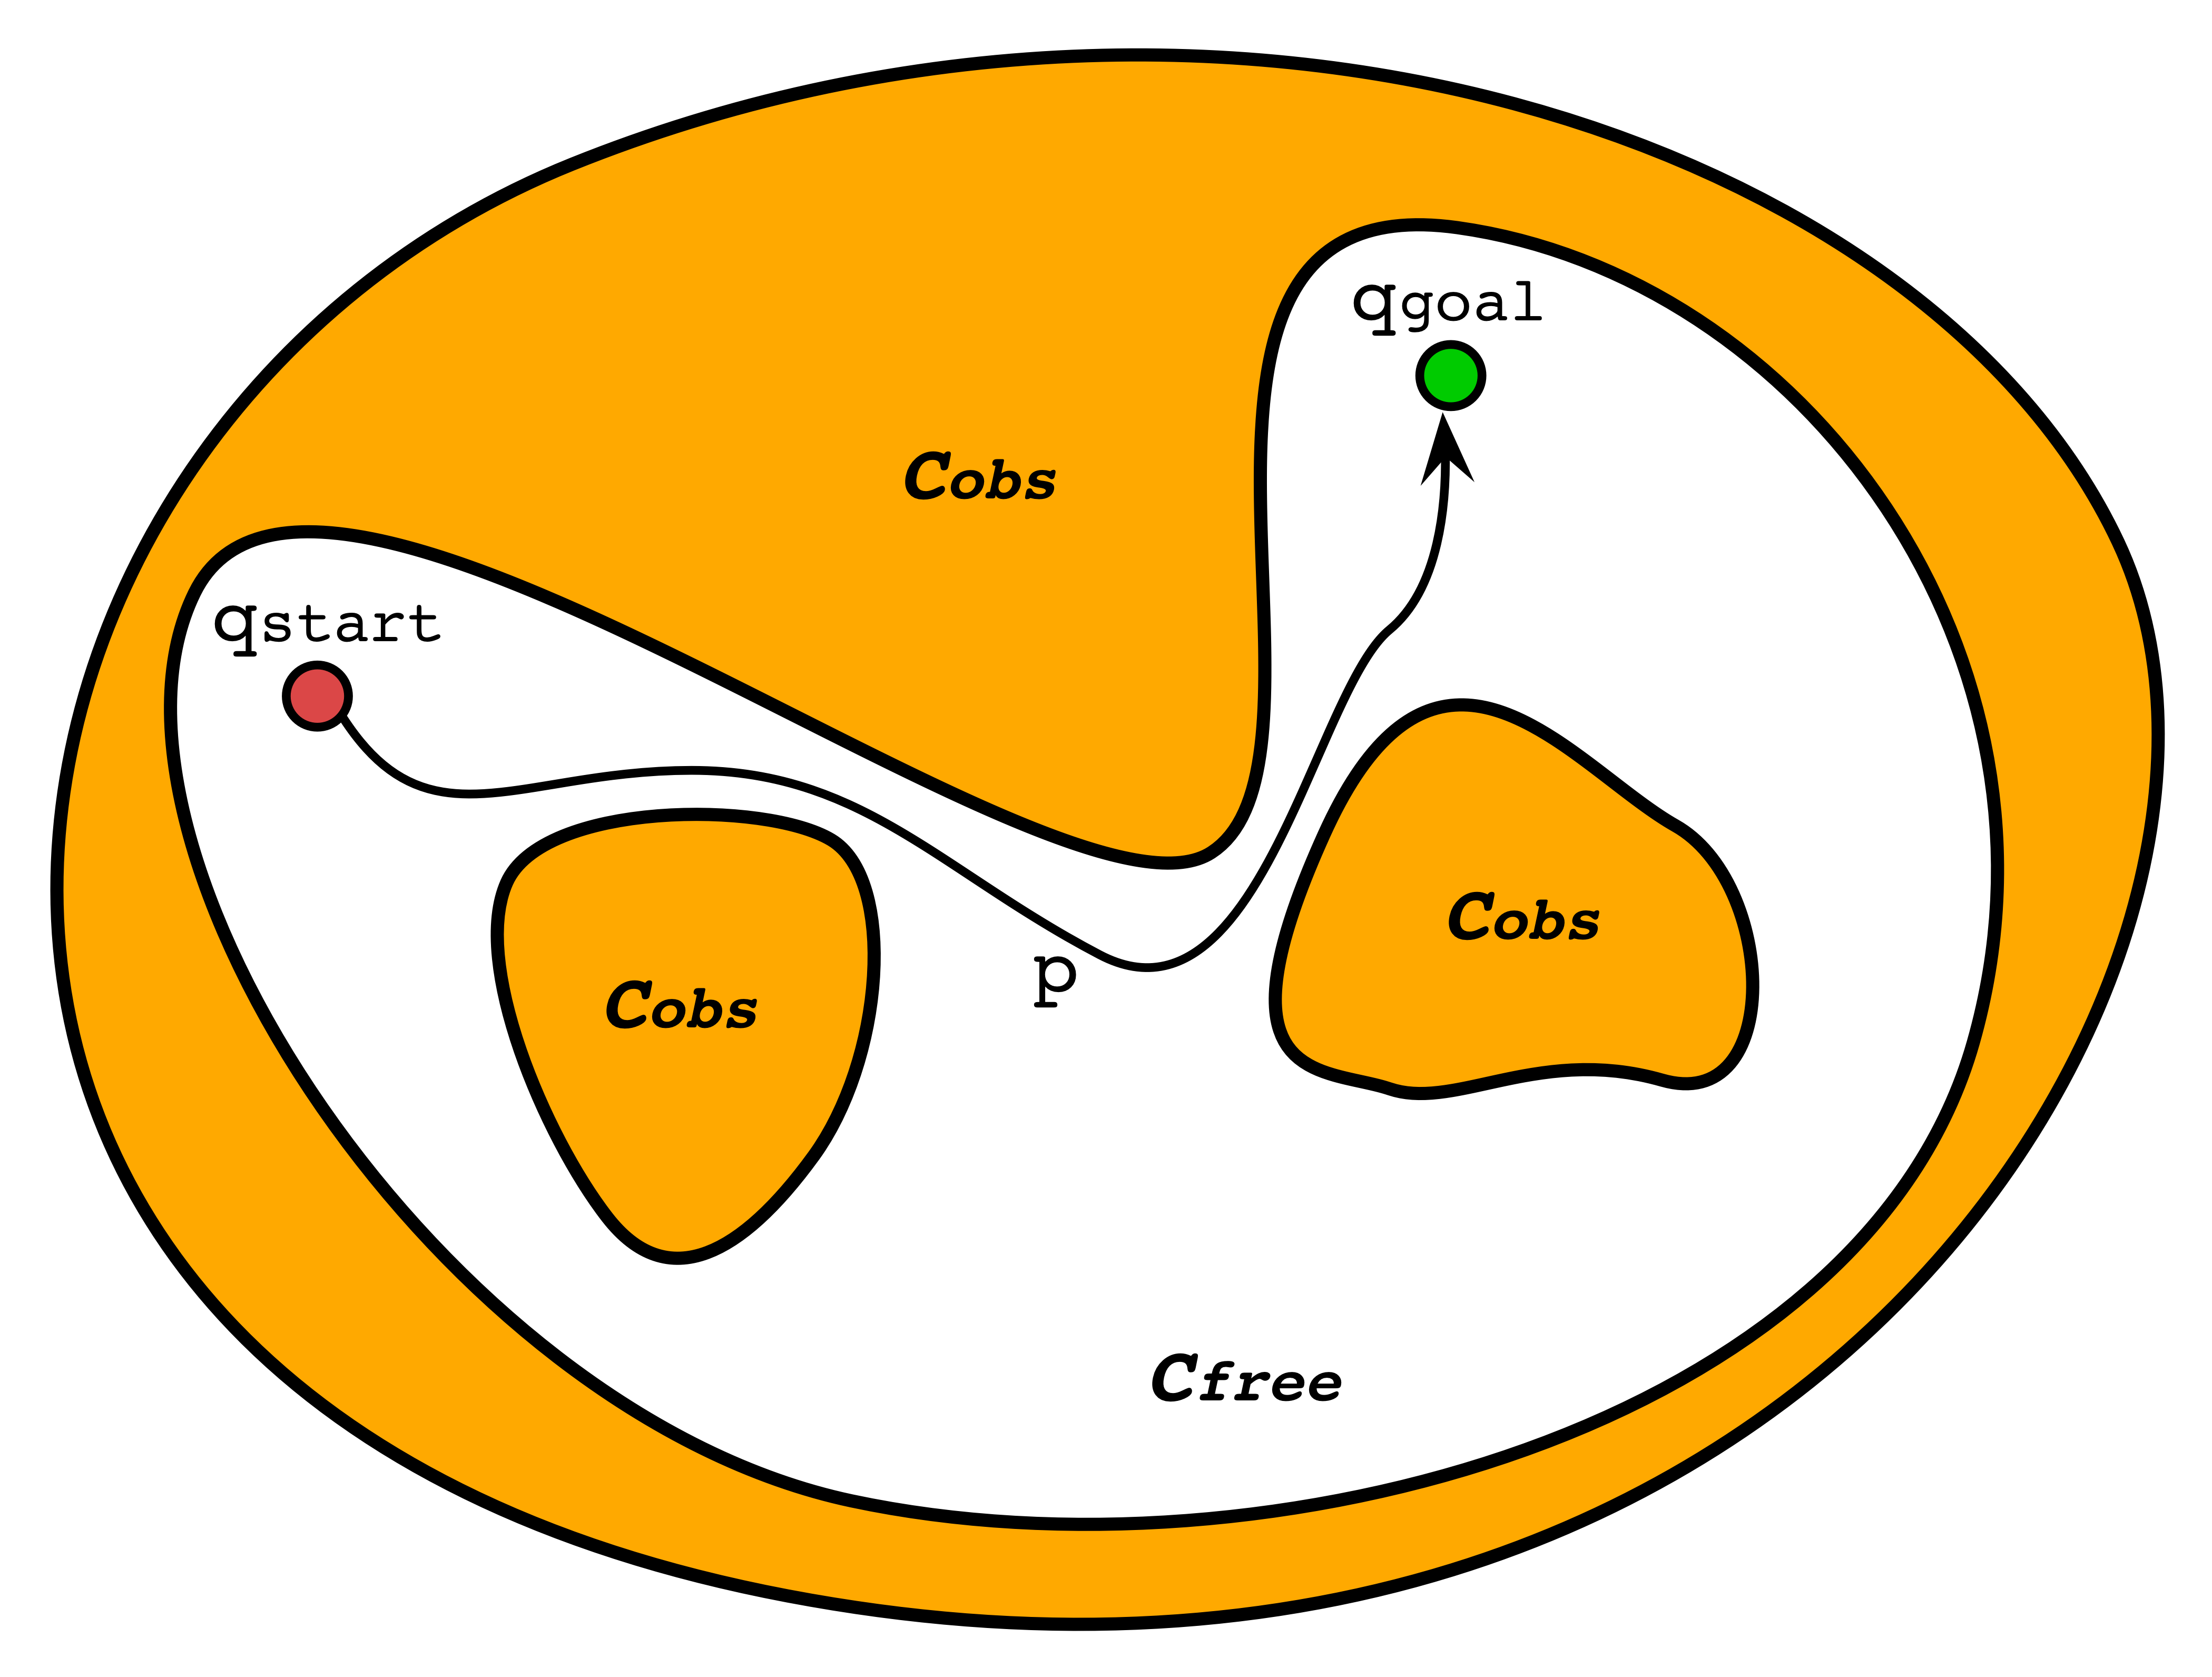
\includegraphics[width=.75\linewidth]{collision-free-path}
\caption[The basic path/motion planning problem and the \ac{C-Space} concept.]
{The basic path/motion planning problem seeks to connect a start configuration
($q_{start}$) and goal configuration ($q_{goal}$) with a continuous
collision-free path $p:[0,1] \rightarrow \mathcal{C}_{free}$.}
\label{fig:collision-free-path}
\end{figure}

% ----------------------- another section  ------------------------
\section{Bug-based Methods}

Bug-based methods represent one of the earliest reactive and sensor-based path
planning approaches, in which a mobile robot moves in the plane towards a global
goal, while having a limited (local) knowledge of the environment. The
algorithms included in this group are based on two basic behaviors: go straight
towards the goal and follow the obstacles' boundary. Lumelsky and Stepanov
presented the first of these algorithms, known as Bug1 and Bug2, that mainly
rely on tactile or zero range sensors to perceive the
obstacles~\cite{Lumelsky1987}. Later, Kamon \etal introduced the Tangent Bug
algorithm, which is an extension that uses non-zero range
sensors~\cite{Kamon1996}. All of them are classified as complete algorithms,
which means that they find a solution when one is possible or, otherwise, they
report when there is no solution. Furthermore, they assume the robot is a point
that moves in a \ac{2D} workspace, and that it is capable of knowing its
position and calculating its distance to the goal.

Bug1~\cite{Lumelsky1987} is the most basic algorithm that uses the
aforementioned behaviors. With this method, the robot moves from the start
position ($q_{start}$) towards the desired goal position ($q_{goal}$) until it
reaches the goal or until it finds an obstacle (detected with its tactile
sensors). When the latter situation occurs, the robot stores its current
position and marks it as the \textit{hit point} ($H_i$). Then it changes its
motion mode (behavior) to completely circumnavigate the obstacle. While the
vehicle follows the obstacle boundary, it continuously calculates the distance
to the goal in order to determine the position that corresponds to the minimum
possible distance. This is marked as the \textit{leave point} ($L_i$). Once the
robot reaches the \textit{hit point} again (\ie after it has traveled all the
obstacle contour), it goes back to the \textit{leave point} and there changes
its behavior, once again, in order to move towards the goal. This procedure is
repeated until reaching the specified goal. Figure~\ref{fig:Bug1} depicts an
example of this algorithm solving a start-to-goal query.

\begin{figure}[htbp]
	\centering
	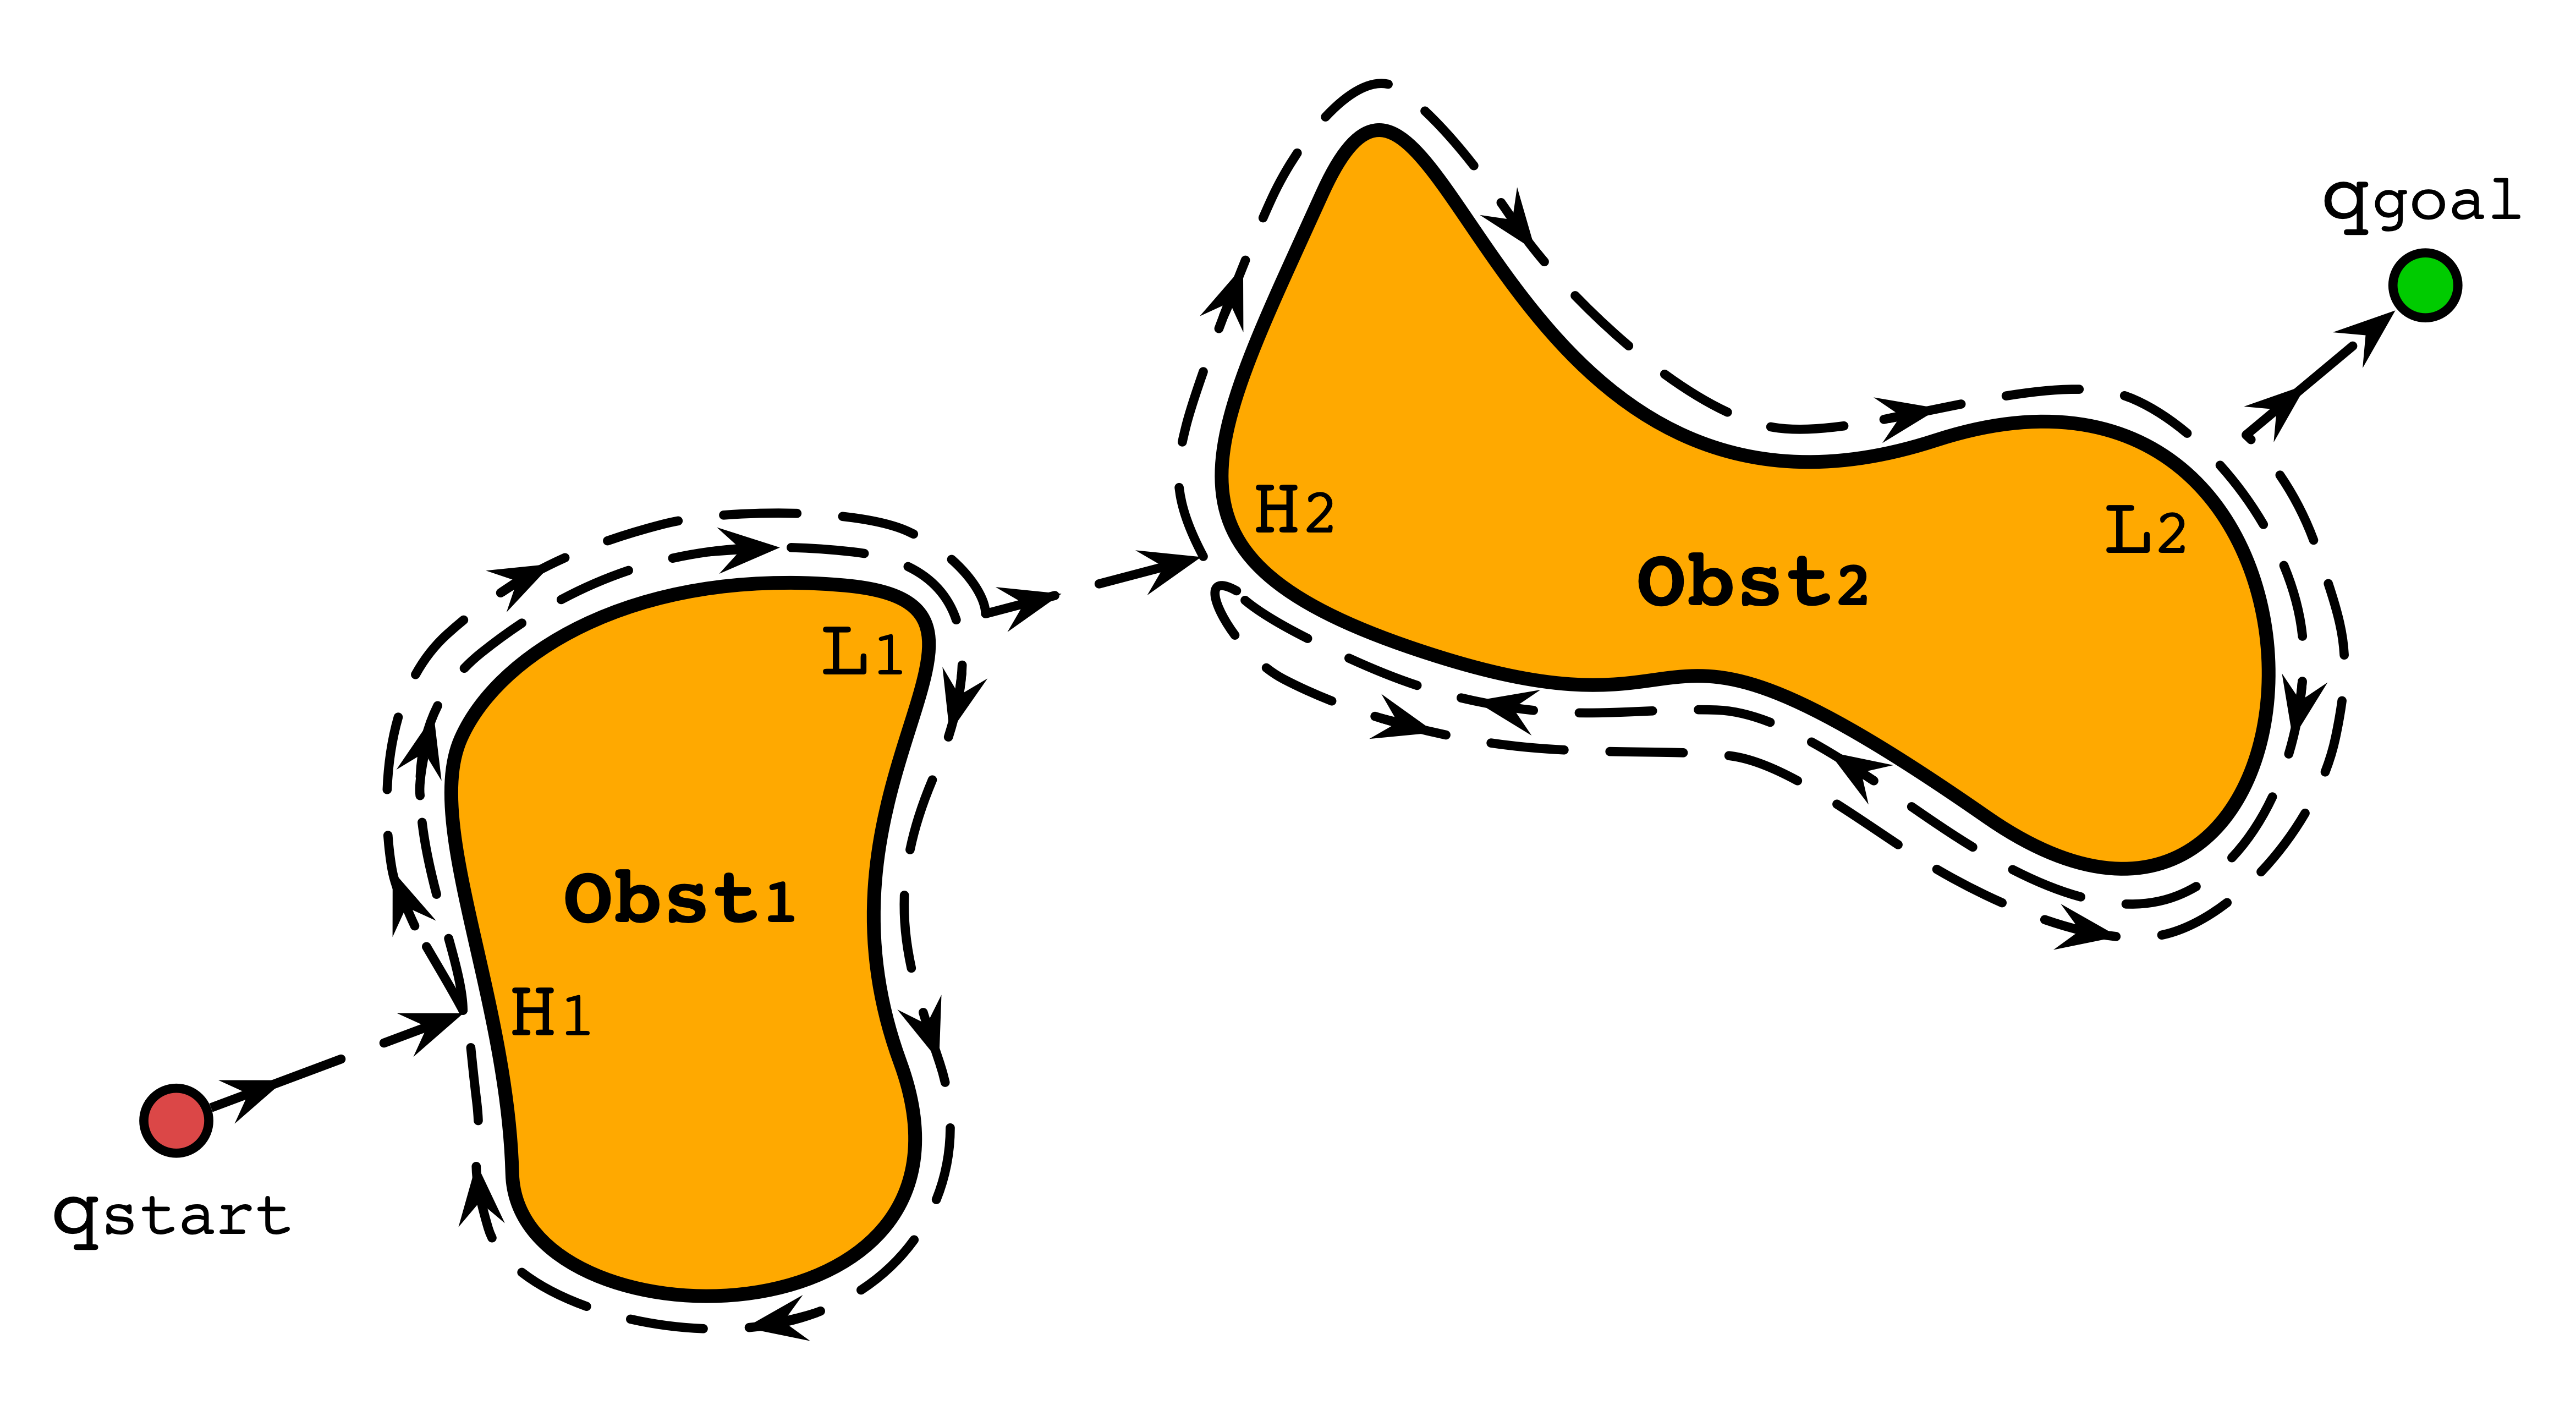
\includegraphics[width=.75\linewidth]{Bug1} \quad
\caption[Reactive and sensor-based method Bug1.]
{Reactive and sensor-based method Bug1}
\label{fig:Bug1}
\end{figure}

Bug2~\cite{Lumelsky1987} attempts to be an improved version of the previously
explained algorithm. It establishes a straight line, sometimes referred as the
\textit{m-line}~\cite{Choset2005}, which connects the start and goal positions.
With this algorithm, the robot starts moving towards the desired goal by
following the \textit{m-line} until it reaches the goal or finds an obstacle. As
occurs with Bug1, if the robot is dealing with an obstacle, it first marks that
position as the \textit{hit point} ($H_i$) and then changes its behavior to
circumnavigate the obstacle. However, with Bug2 the robot does not necessarily
travel the entire obstacle boundary, but instead stops when reaching another
point in the \textit{m-line}; if such a point is closer to the goal than the
previous \textit{hit point}, the robot marks this position as \textit{leave
point} ($L_i$) and, from there, continues following the \textit{m-line} towards
the goal. This procedure is repeated until reaching the specified goal. Even
though Bug2 does not require to completely circumnavigate the obstacles, there
are environments where the robots do require to travel the entire boundary; in
these cases Bug2 may generate longer paths than those calculated by Bug1, and
therefore is less efficient. Figure~\ref{fig:Bug2} depicts an example of Bug2
solving start-to-goal queries in both simple and complex scenarios.

\begin{figure}[htbp]
    \myfloatalign
    \subfloat[Bug2 simple scenario]
    {\label{fig:Bug2-simple}
    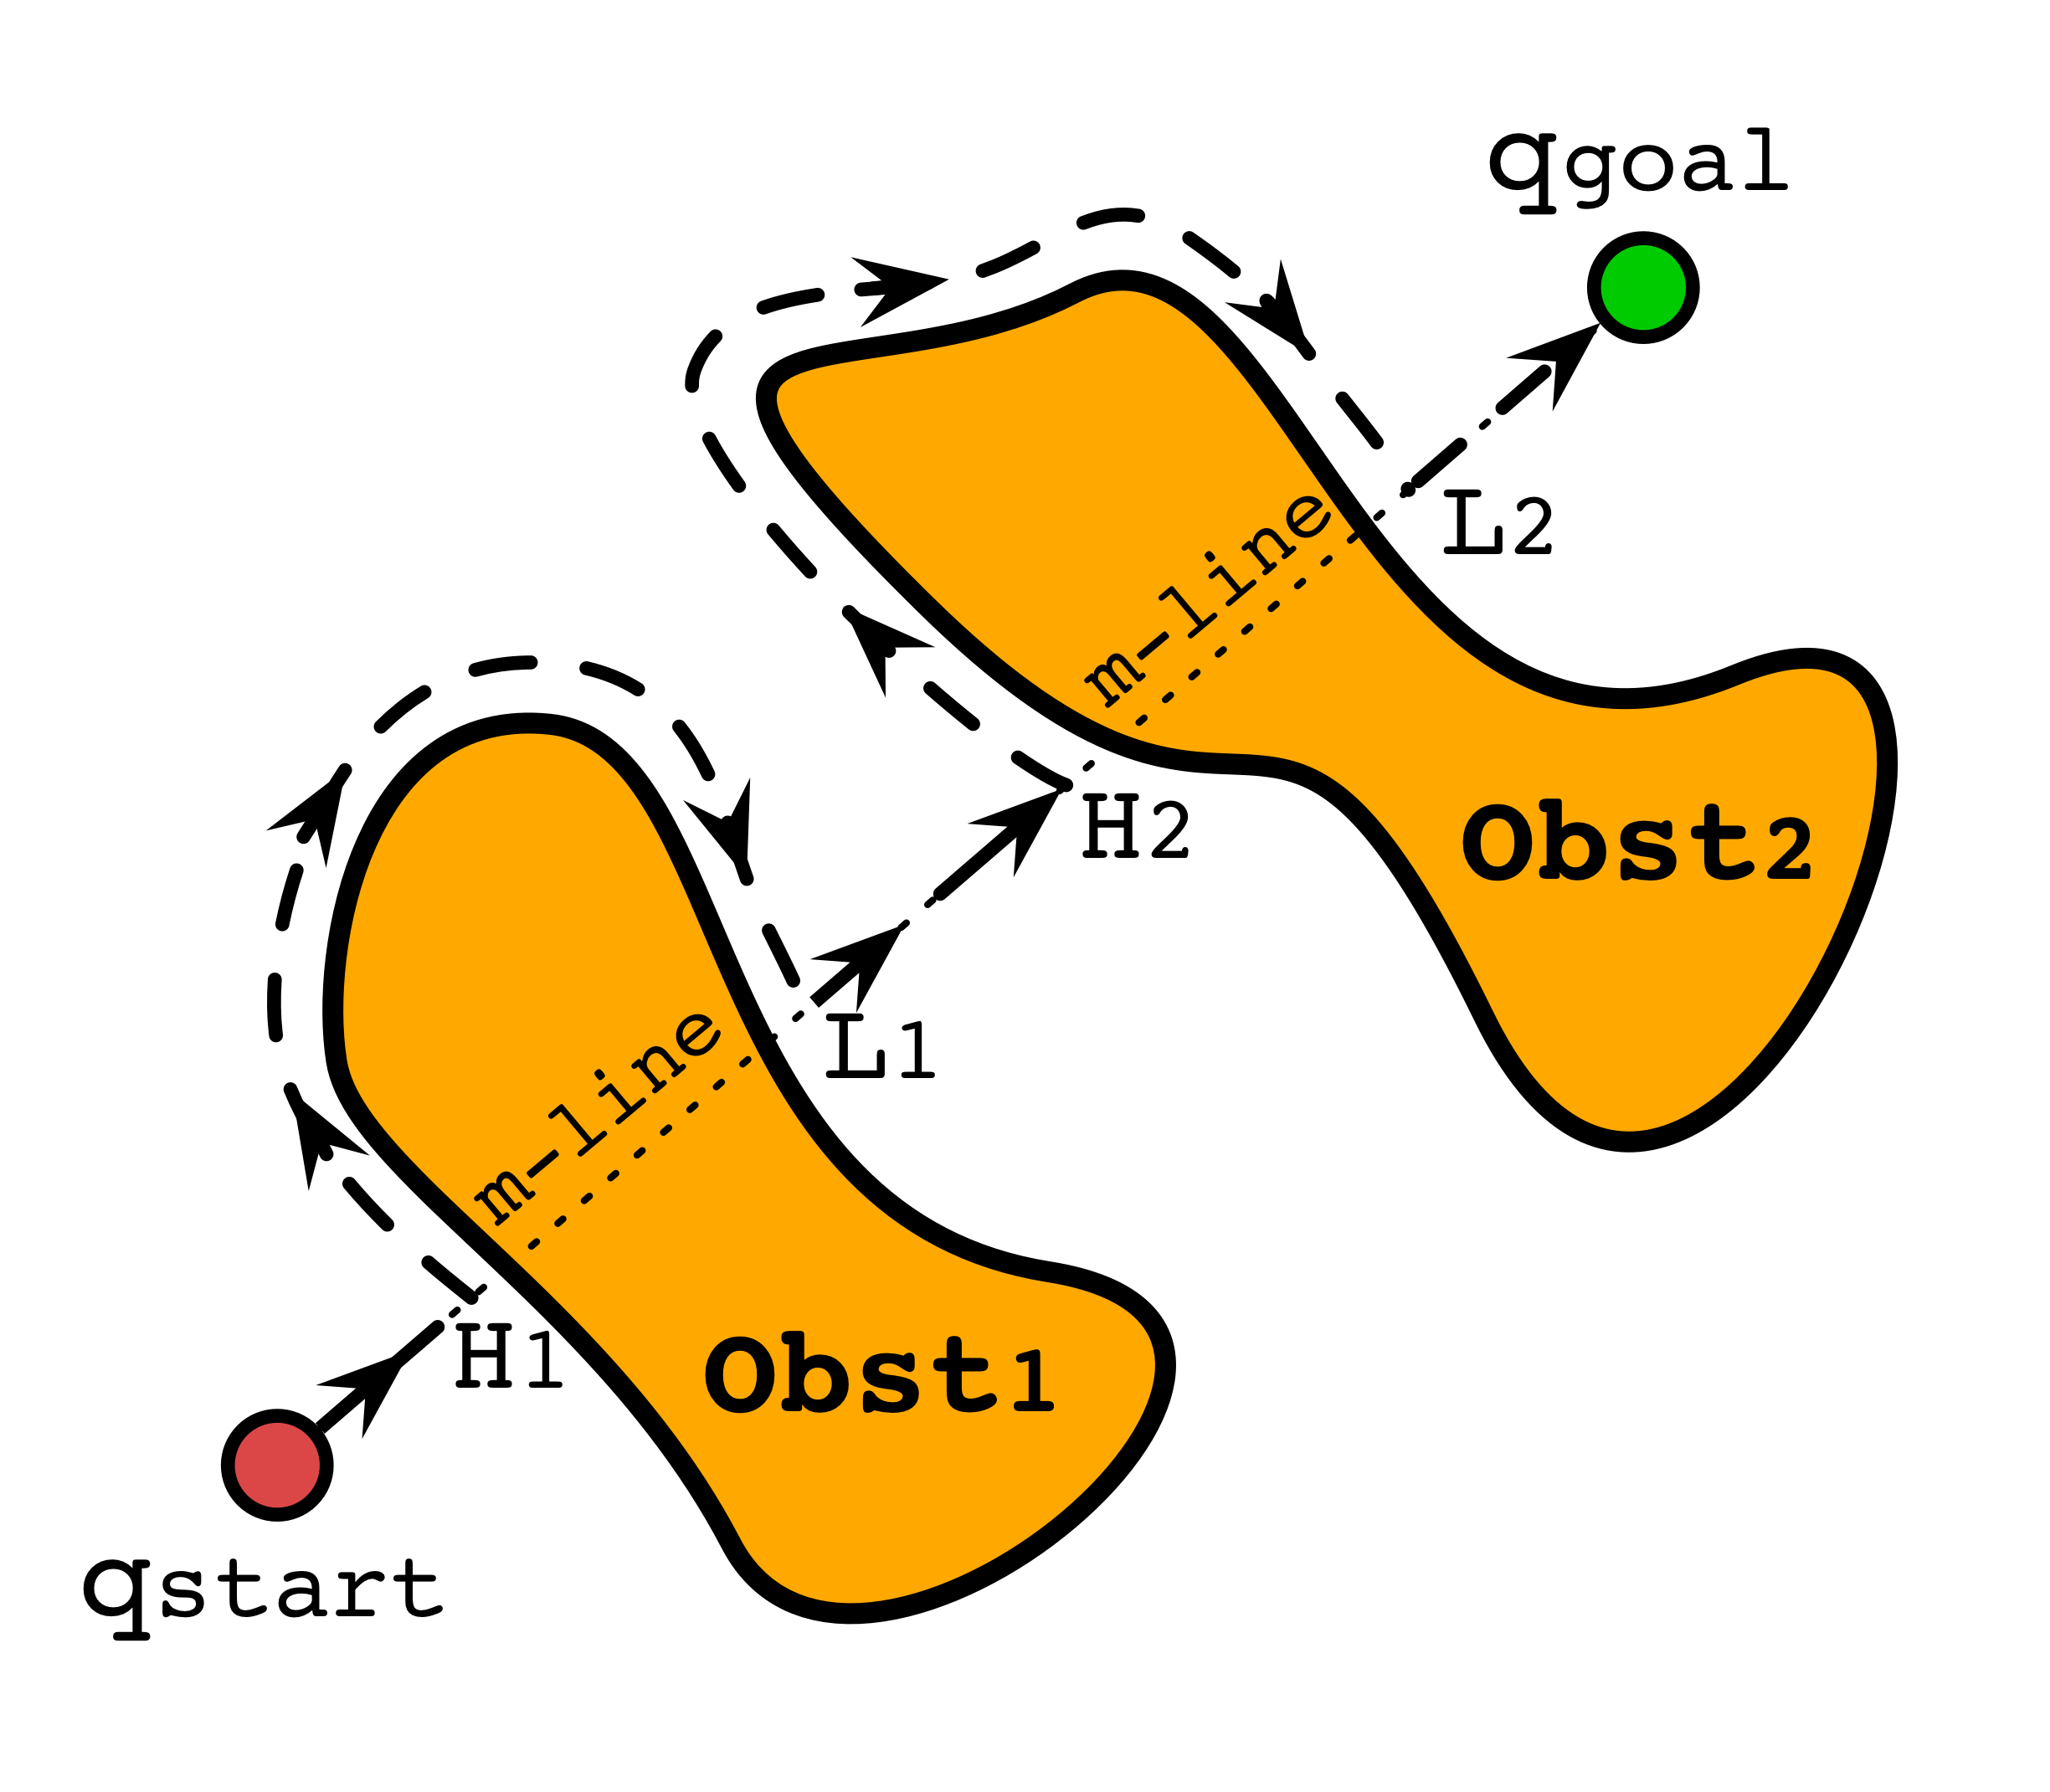
\includegraphics[width=.48\linewidth]{Bug2}} \quad
    \subfloat[Bug2 complex scenario]
    {\label{fig:Bug2-complex}%
     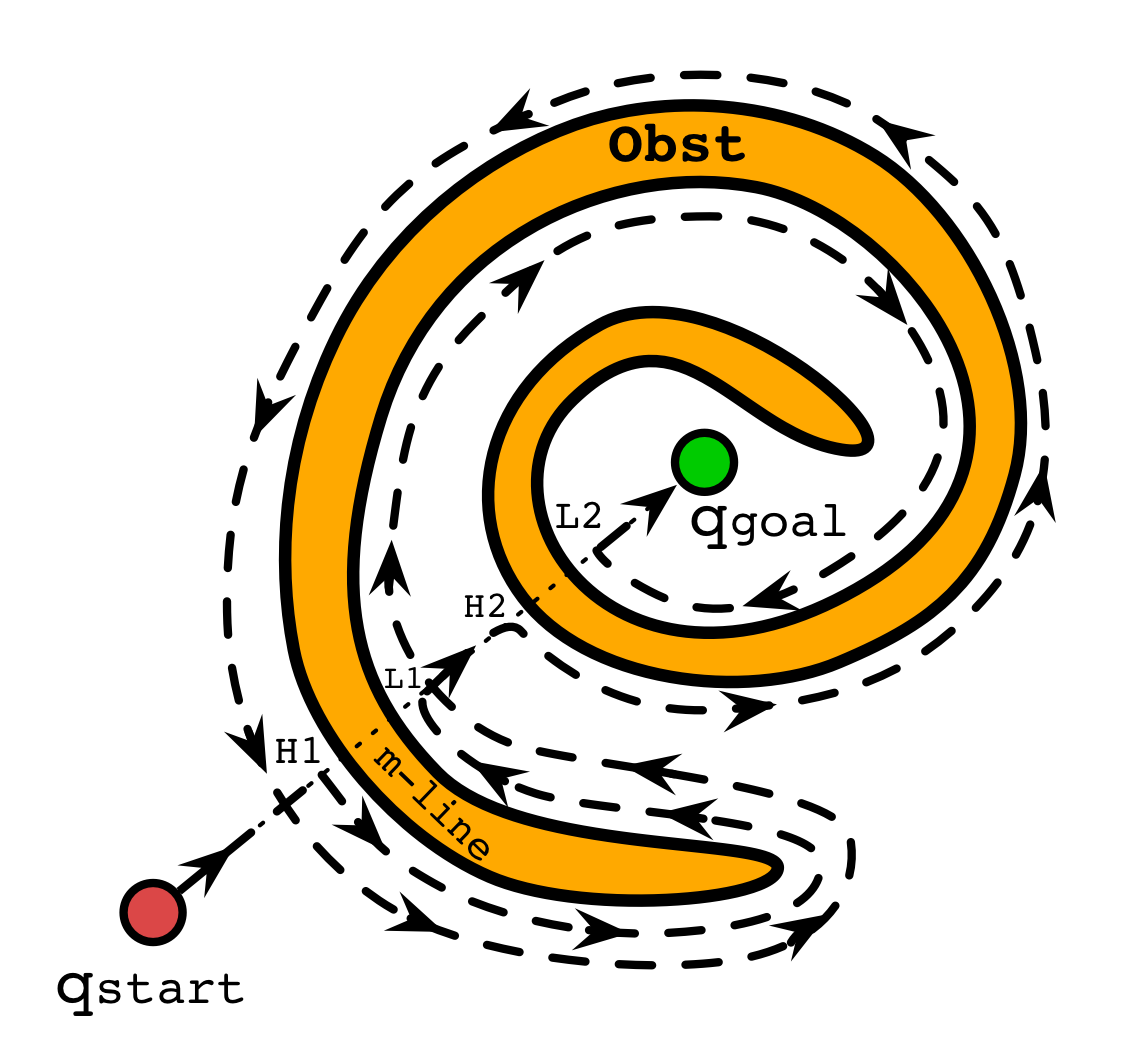
\includegraphics[width=.48\linewidth]{Bug2-complex}}
\caption[Reactive and sensor-based method Bug2.]
{Reactive and sensor-based method Bug2}
\label{fig:Bug2}
\end{figure}
 
Finally, the Tangent Bug algorithm~\cite{Kamon1996} was proposed as an improved
alternative for Bug1 and Bug2. In this version, the robot is assumed to be
equipped with a non-zero range sensor, which permits detecting in advance not
only the obstacles, but also their continuous boundaries. This way, when the
robot is navigating towards the goal and faces an obstacle, it can determine the
discontinuities in the boundaries or the limits of the perceived area, which are
marked as \textit{endpoints}. Then, in order to avoid the obstacle, the robot
checks which of the \textit{endpoints} minimizes the distance to the goal and
starts moving towards it. The procedure is repeated until the obstacle is no
longer perceived, at which point the robot can continue moving towards the goal
following a straight line. Figure~\ref{fig:TangentBug} depicts an example of
Tangent Bug solving a start-to-goal query.
 
\begin{figure}[htbp]
    \myfloatalign
    \subfloat[Boundaries detection]
    {\label{fig:TangentBug-Boundaries}
    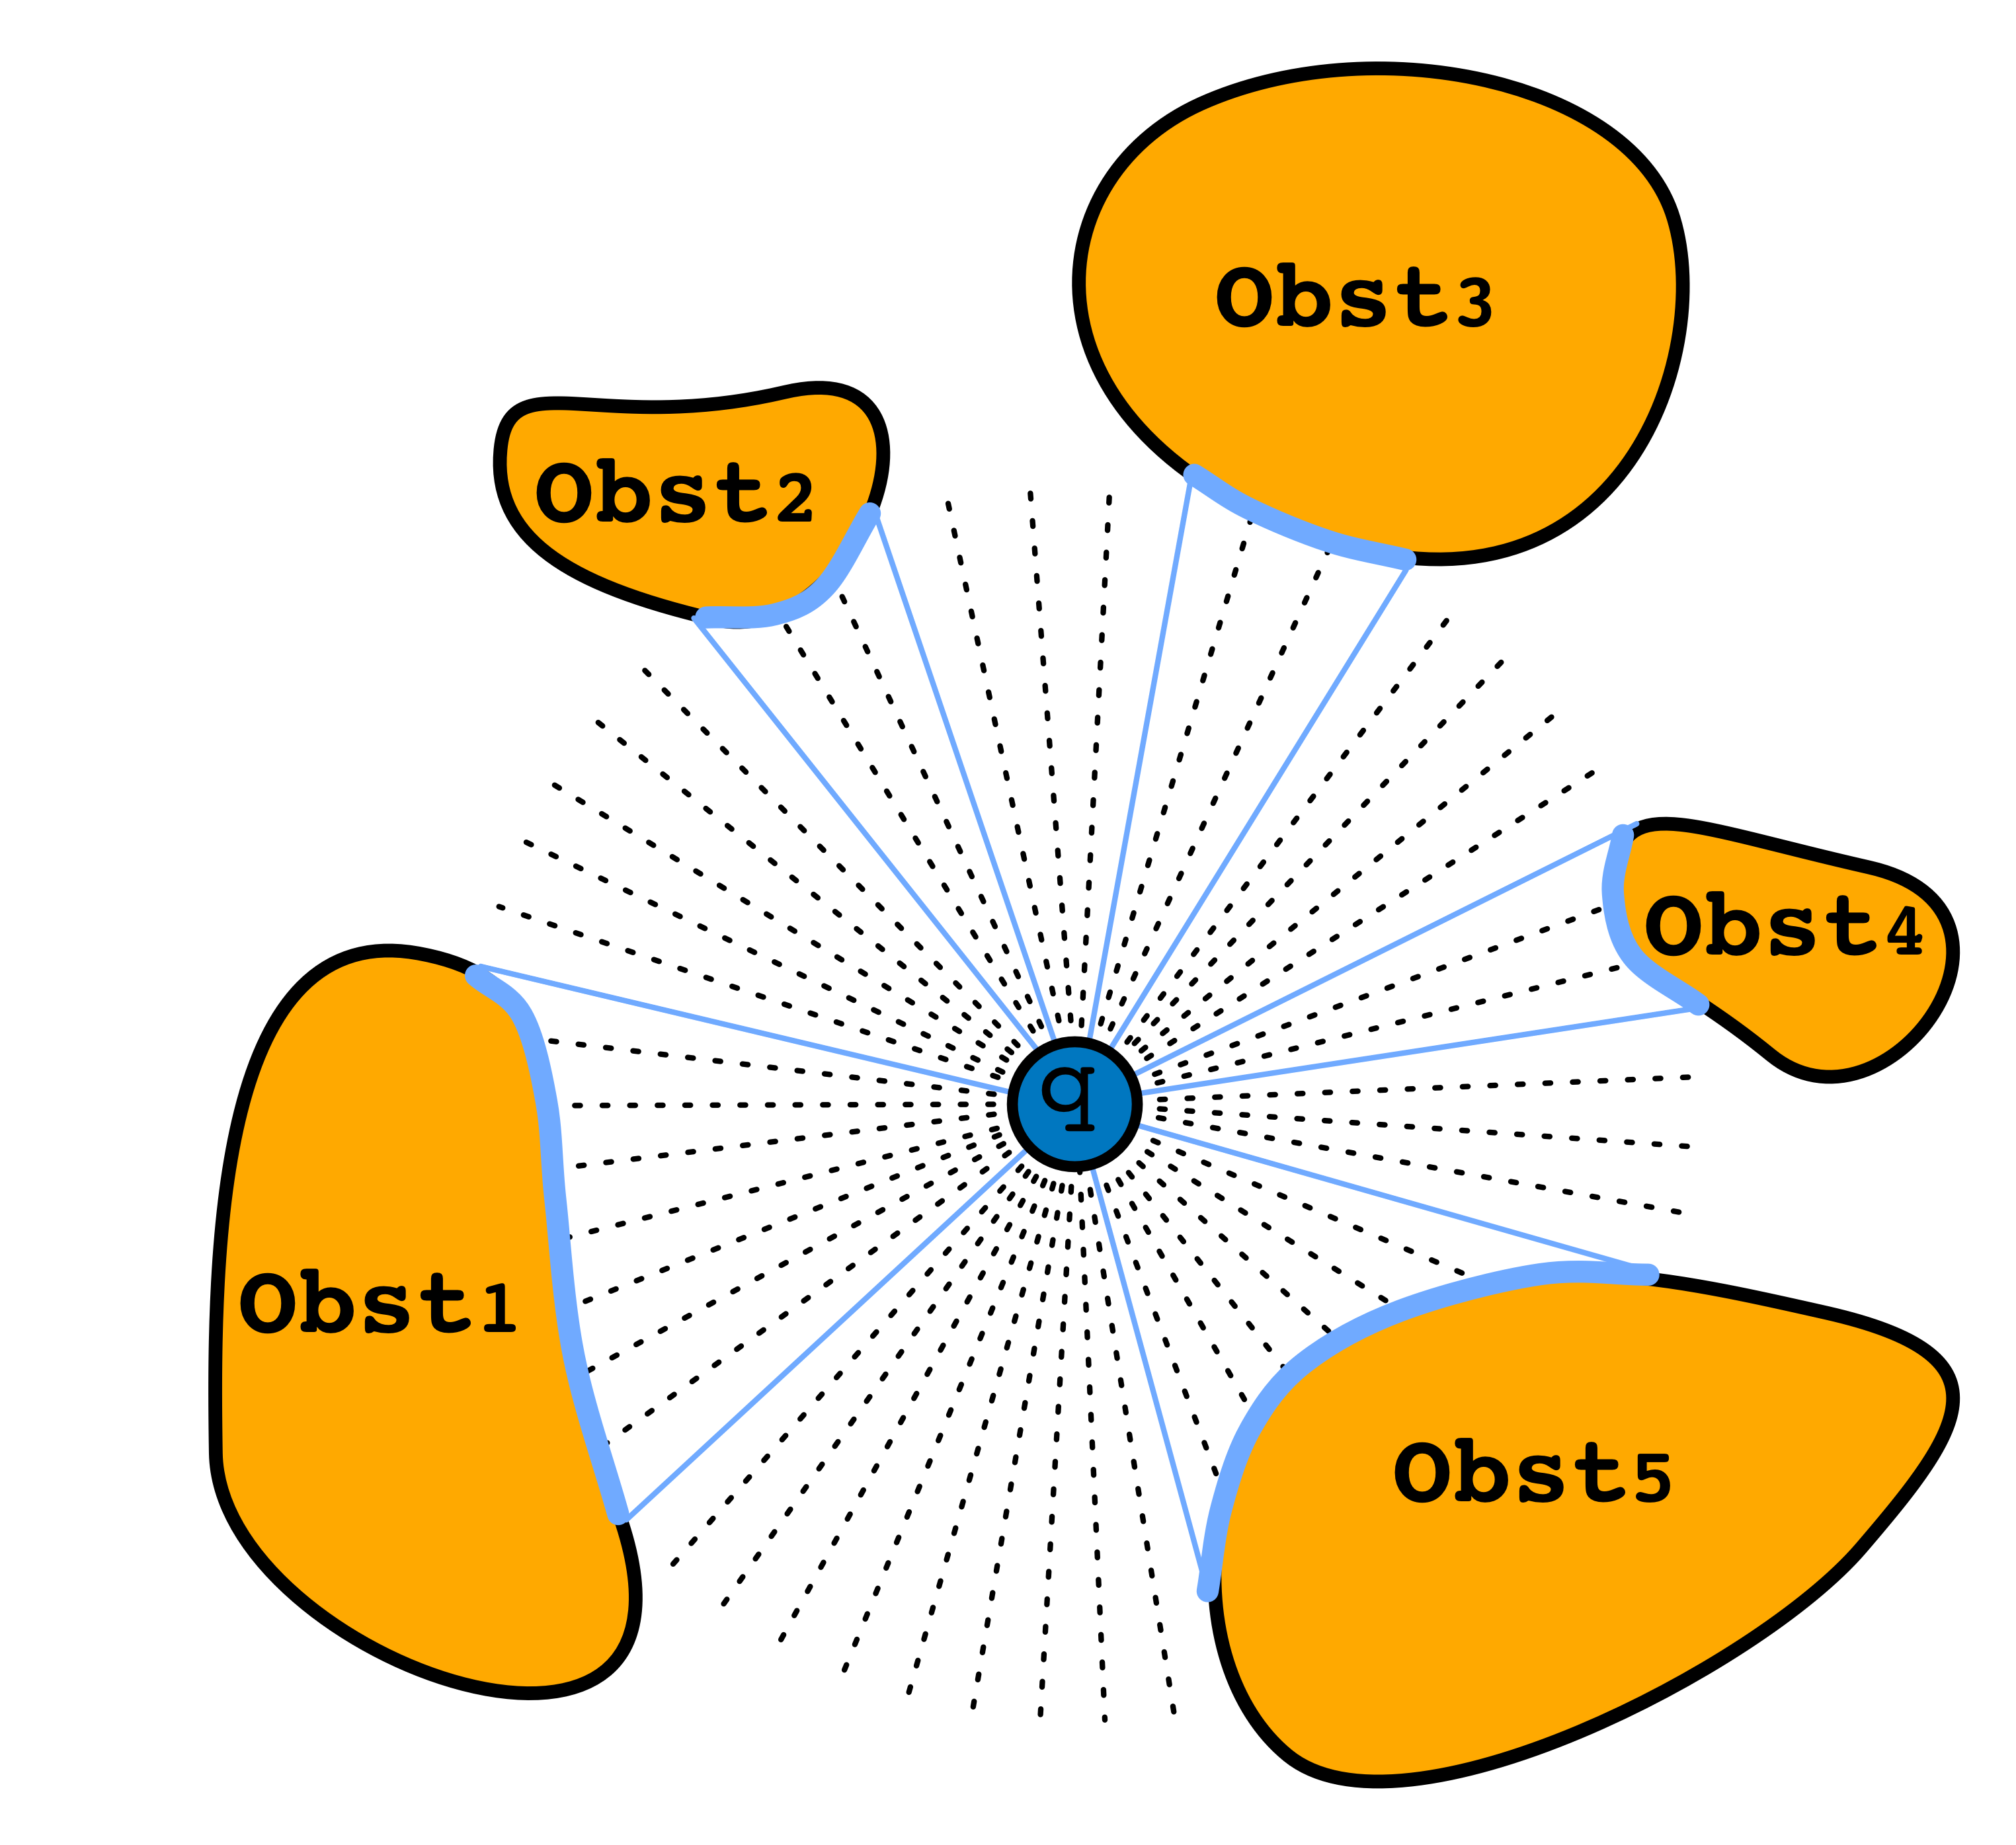
\includegraphics[width=.48\linewidth]{TangentBug-Boundaries}} \quad
    \subfloat[Execution]
    {\label{fig:TangentBug-Execution}%
     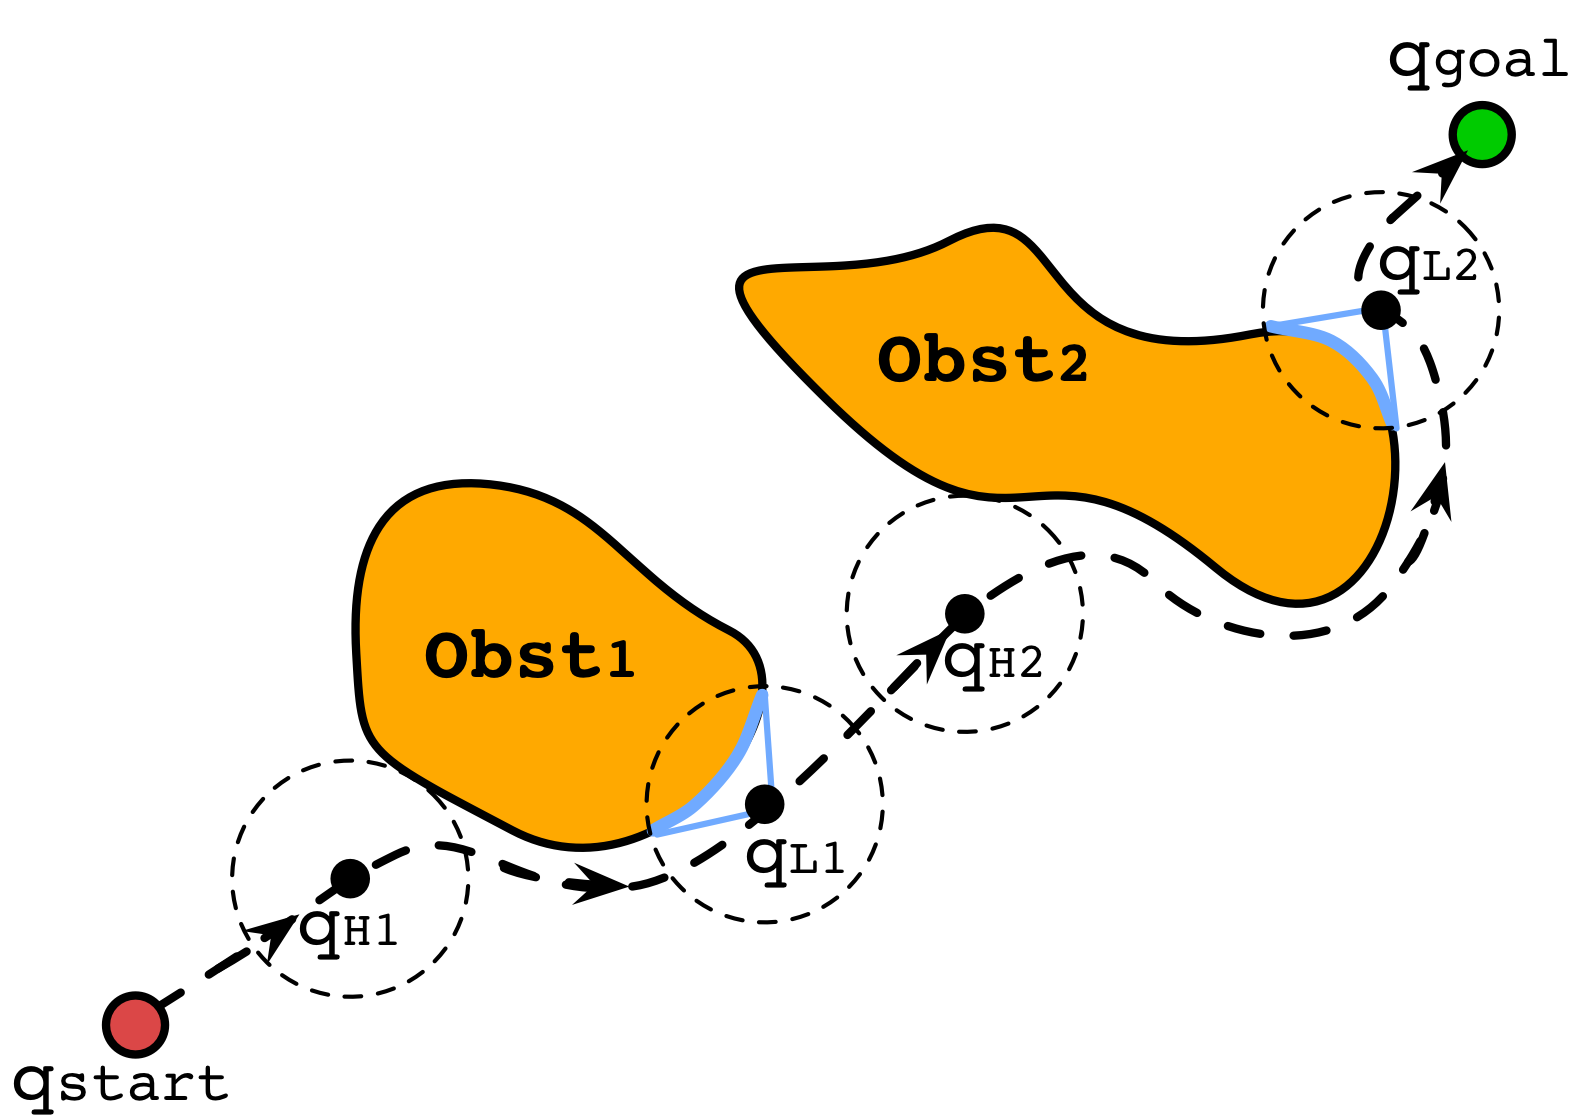
\includegraphics[width=.48\linewidth]{TangentBug-Execution}}
\caption[Reactive and sensor-based method Tangent Bug.]
{Reactive and sensor-based method Tangent Bug}
\label{fig:TangentBug}
\end{figure}

% ----------------------- another section  ------------------------=
\section{Search-based (Grid-based) Path Planning}
\label{sec:SearchBased}

Search-based planning is a path planning approach that utilizes graph search
methods to find collision-free paths over a discrete version of $\mathcal{C}$.
For doing so, these methods overlay a grid on $\mathcal{C}$ and assume that each
collision-free configuration corresponds to a point on the grid, which is why
they are also called grid-based methods. Over that grid, the robot is allowed to
move from one point to any other adjacent point as long as the line between them
is proved to be collision-free (\ie is contained within $\mathcal{C}_{free}$).
Hence, using this approach to solve, for instance, a start-to-goal query
requires coping with two problems: how to correctly discretize $\mathcal{C}$ to
establish the grid, and how to search a path from the start point to the goal
point (configuration) over such a grid.

For the first problem, it is important to correctly define the grid resolution,
which mainly depends on the environment and the problem's requirements. Coarser
grids, for example, will permit faster searches, but may fail to find paths when
dealing with narrow passages in $\mathcal{C}_{free}$ (see
Figure~\ref{fig:Grid-based}). Finner grids, on the other hand, will allow
solving queries in more complex scenarios, but may be computationally too
expensive for online applications. Once the grid is established, there are
different methods to calculate an optimal path, some of which are described in
this section.

\begin{figure}[htbp]
    \myfloatalign
    \subfloat[Coarse grid]
    {\label{fig:Grid-BasedNarrowPassagesNoValid}%
     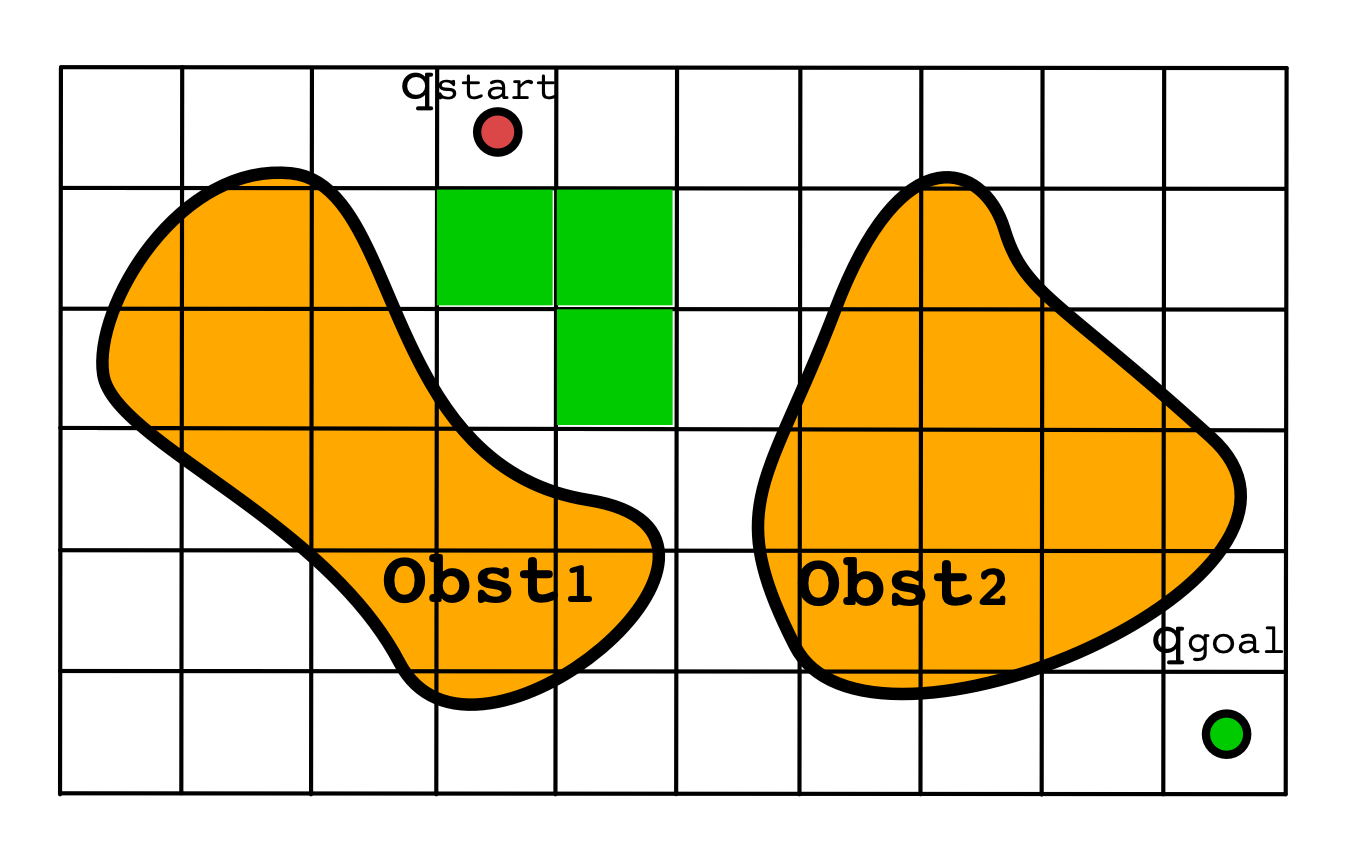
\includegraphics[width=.48\linewidth]{Grid-BasedNarrowPassagesNoValid}} \quad
    \subfloat[Fine grid]
    {\label{fig:Grid-BasedNarrowPassagesValid}
    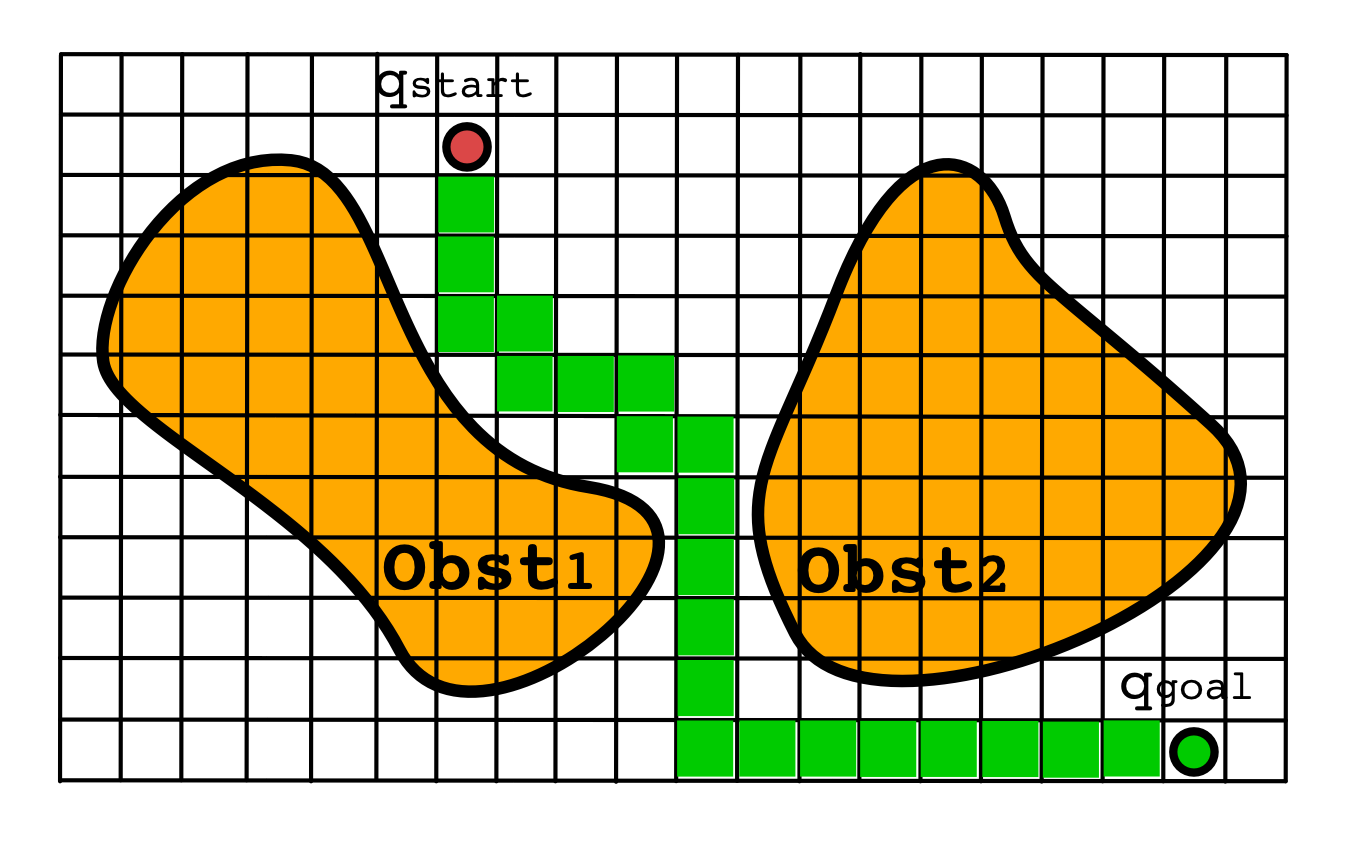
\includegraphics[width=.48\linewidth]{Grid-BasedNarrowPassagesValid}}
\caption[Grid-based method: coarse and fine grid.]
{Grid-based method solving a start-to-goal query.
\protect \subref{fig:Grid-BasedNarrowPassagesNoValid} Although coarser grids
decrease the computing time, they may fail when dealing with narrow passages
where finer grids could succeed \protect
\subref{fig:Grid-BasedNarrowPassagesValid}.}
\label{fig:Grid-based}
\end{figure}

\subsection{Dijkstra's Algorithm}

Presented in 1959, Dijkstra's algorithm~\cite{Dijkstra1959} is one of the first
widely known methods used to find a path in a graph from one node to another.
The algorithm uses a weighted graph $\mathcal{Q}$\footnote{A weighted graph is
one in which numerical values, or weights, are assigned to its nodes and edges.}
to determine which path that connects two nodes has of the lowest cost. While
this method has been used in different areas and applications such as network
routing protocols, in robotics it has been applied to path planning problems.
There, the associated edge cost may correspond to different optimization metrics
such as distance, energy, time, etc., that can be considered when calculating
the optimal path for a start-to-goal query.

In order to find the optimal path, the algorithm iteratively executes the
following steps until reaching the goal ($q_{goal}$):
\begin{inparaenum}[1)] \item Setting an initial cost to all nodes, specifically
zero to the initial one ($q_{start}$) and infinity to all others.
\item Establishing $q_{start}$ as the current node and marking the rest as
unvisited.
\item Calculating the cost for the current node's unvisited neighbors (equal to
the current node's cost plus the edge to the neighbor cost), as well as updating
any previously calculated node cost if the new value is lower.
For example, if node $B$ cost was $x$ when current node was $A$, but the new
cost is $y$ when current node is $C$, and $y<x$, then node $B$ cost will be now
$y$.
\item After calculating the cost of all its unvisited neighbors, current
node is marked as visited.
\item If the $q_{goal}$ has been marked as visited, the algorithm has finished,
otherwise, the new current node will be the unvisited node with the lowest
cost, and will be processed as indicated from step 3).
\end{inparaenum}
Finally, the least cost path can be obtained with backtracking.
Figure~\ref{fig:Dijkstra} presents an example of executing this method.

\subsection{A*}

In 1968, Peter Hart \etal described an extension of Dijkstra's algorithm called
A*~\cite{Hart1968}, which incorporates a heuristic that permits estimating the
cost of paths from any node of the graph to the goal. Because of this
characteristic, A* is considered an informed search algorithm; this means that
it always attempts to find the path by firstly evaluating those nodes with the
minimum estimated cost according to the heuristic. As occurs with Dijkstra's
algorithm, A* starts from a weighted graph $\mathcal{Q}$, in which each node
represents a different configuration contained in $\mathcal{C}_{free}$ and the
edges correspond to collision-free paths between configurations. Then, it builds
a search tree, rooted at $q_{start}$, by expanding different paths, one step at
a time, until one of them ends at the desired $q_{goal}$. The main difference
with respect to Dijkstra's algorithm is the order in which each partial path is
expanded. In the case of A*, it expands the node $q_i$ that minimizes the total
cost $f(q_i) = g(q_i) + h(q_i)$, which combines the cost required to reach the
node from the start configuration $g(q_i)$ with the estimated heuristic cost
from the node to the goal $h(q_i)$.

While both Dijkstra's algorithm and A* can generate optimal solutions, the
latter can result in a more efficient search by reducing the number of nodes
required to be visited in order to determine the solution path (see
Figure~\ref{fig:Astar}). However, it is important to know that an
incorrect heuristic will also provide a valid solution, but it may be
suboptimal. For this reason and in order to produce an optimal path, the
heuristic has to be optimistic, or admissible, which means that the estimated
cost to the goal has to be lower or equal to the real cost~\cite{Choset2005}.
Finally, it is also important to note that in case no heuristic is provided, \ie
$h(q_i)=0$, A* behaves as Dijkstra's algorithm. Algorithm~\ref{alg:A-star}
presents the pseudocode for A* and also provides a general idea for Dijkstra's
algorithm explained in the previous section.

\begin{figure}[htbp]
    \myfloatalign
    \subfloat[Dijkstra algorithm]
    {\label{fig:Dijkstra}%
     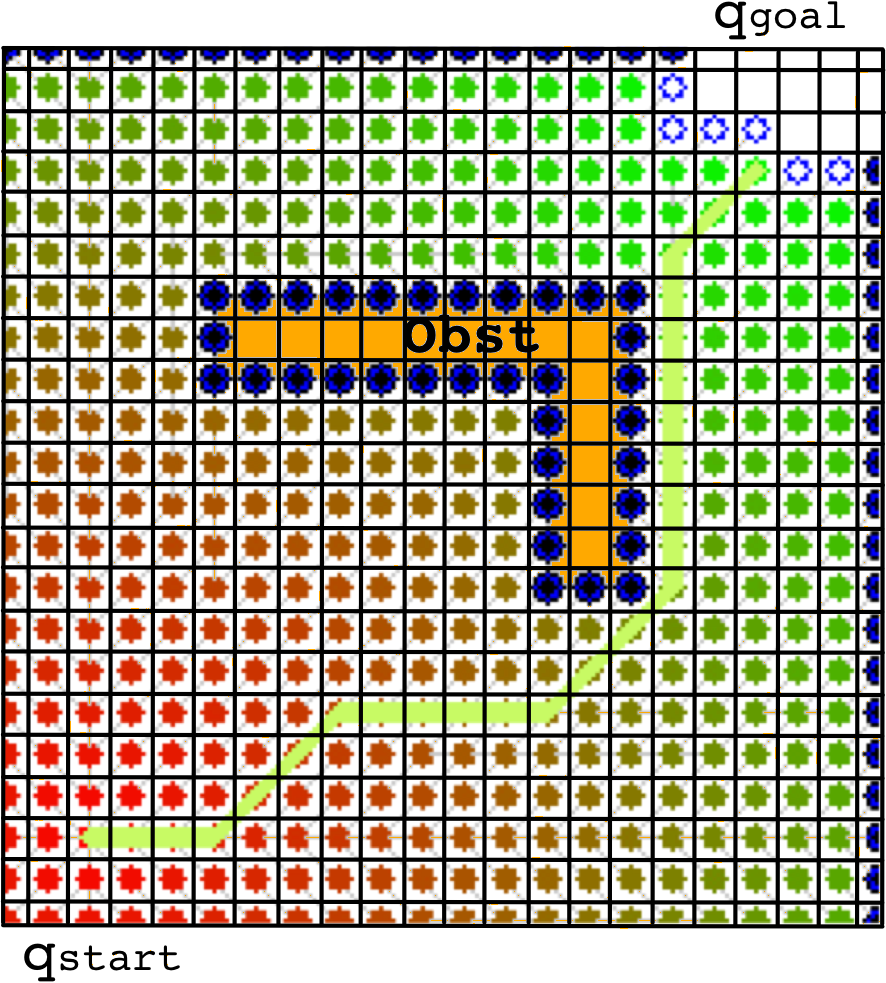
\includegraphics[width=.48\linewidth]{Dijkstra}} \quad
    \subfloat[A*]
    {\label{fig:Astar}
    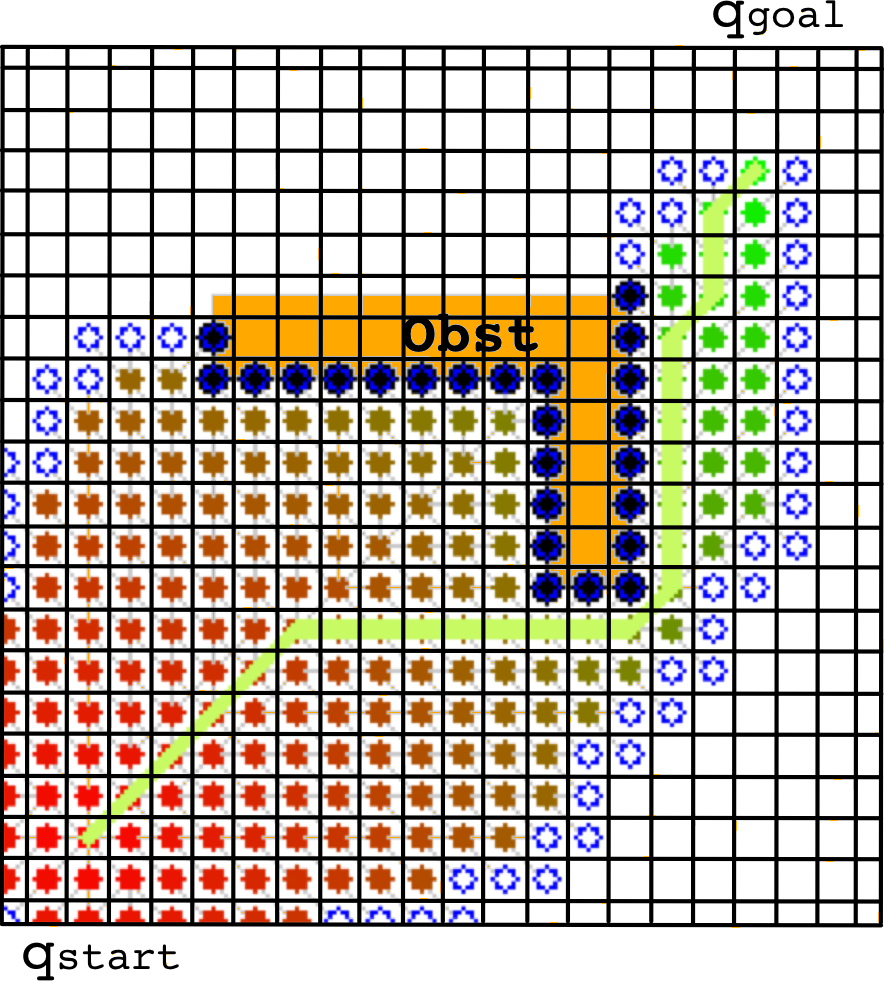
\includegraphics[width=.48\linewidth]{Astar}}
\caption[Comparison between Dijkstra's algorithm and A*.]
{Grid-based methods solving a start-to-goal query.
\protect \subref{fig:Dijkstra} Dijkstra's algorithm requires an exhaustive
search to determine the shortest path to the goal.
\protect \subref{fig:Astar} A* requires exploring less cells since it uses a
heuristic to guide the search. Image credit: modified from Wikipedia.}
\label{fig:Dijkstra-Astar}
\end{figure}

\begin{algorithm}[htbp]
	\DontPrintSemicolon
	\SetKwFunction{popWithMinCost}{popWithMinCost}
	\SetKwFunction{PriorityQueue}{PriorityQueue}
	\SetKwFunction{insertQ}{insert}
	\SetKwFunction{Neighbors}{Neighbors}

	\KwIn{\\ 
	$q_{start}$: Start configuration.\\
	$q_{goal}$: Goal configuration.\\
	$\mathcal{Q}$: Graph of configurations $q$, such that $q \in \mathcal{C}_{free}$}

 	\Begin{
 		\ForAll{$q \in \mathcal{Q}$}{
 			$g(q) = \infty$\;
 		}
 		$g(q_{start}) = 0$\\
 		UNVISITED = \PriorityQueue{}\\
 		UNVISITED.\insertQ{$q_{start}$, $g(q_{start})+h(q_{start}, q_{goal})$}\\
 		\While{$\argmin\limits_{q \in UNVISITED} (g(q)+h(q, q_{goal})) \neq
 		q_{goal}$}{
 			$q \leftarrow$UNVISITED.\popWithMinCost{}\\
 			\ForAll{$q' \in \mathcal{Q}.\Neighbors{q}$}{
	 			\If{$g(q')>g(q)+c(q,q')$}{
	 				$g(q') = g(q) + c(q,q')$\\
	 				UNVISITED.\insertQ{$q'$, $g(q')+h(q', q_{goal})$}\\
 				}
	 		}
 		}
 	}
 \caption{A*}
 \label{alg:A-star}
\end{algorithm}

\subsection{Dynamic A* (D*)}
\label{sec:D-star}

The aforementioned search-based algorithms, at least in their original versions,
are intended for planning paths in static environments. Nonetheless, there are
situations, especially in mobile robotics applications, in which elements of the
environment may change. For those cases, Anthony Stentz proposed the
\ac{D*}~\cite{Stentz1994,Stentz1995}, an incremental search-based algorithm that
plans collision-free paths using a similar strategy as A*. The difference is
that it also allows to replan according to changes observed in the surroundings
while the robot follows the path to the goal. Its most important characteristic
is that it locally repairs the path, which is more efficient that invoking
multiple times A* to find a new valid path. Contrary to Dijkstra's algorithm and
A*, that both search paths from the start to the goal configuration, \ac{D*}
expands nodes by searching backwards from the goal until the node to be expanded
coincides with the start configuration, at which time the search is concluded.
At the moment, \ac{D*} and some of its variants are probably the most used
search-based methods in mobile robotics. Some of those extensions and
applications will be presented in Section~\ref{sec:ExtensionsApplications}.

% ----------------------- another section  ------------------------
\section{Potential Fields}
\label{sec:PotenFields}

Even though search-based methods have proved to be successful in \ac{2D} and
\ac{3D} workspaces for some terrestrial, aerial and even aquatic robotic
applications, those exhaustive methods suffer from scalability issues in
problems involving high-dimensional configuration spaces. Another important
drawback is the necessity of establishing a grid over $\mathcal{C}_{free}$,
which means discretizing the \ac{C-Space}, thus limiting the possible and
available solutions according to the chosen resolution. An alternative approach
is the use of potential functions.

Originally proposed by Oussama Khatib in 1985~\cite{Khatib1985,Khatib1986},
potential functions, also known as \textit{potential fields}, constitute a
reactive approach for path planning, which attempts to guide a robot from an
initial configuration to a goal configuration while avoiding obstacles. A
\textit{potential field} basically defines a real-valued function $U:
\mathbb{R}^m \rightarrow \mathbb{R}$, which is composed of an attractive
component $U_a(q)$ that pulls the robot towards the goal, and a repulsive
component $U_r(q)$ that pushes the robot away from the obstacles. This function
can be viewed as the total energy $U(q) = U_a(q) + U_r(q)$, which means that the
total force applied by the potential field to the robot is defined as the
negative of the vector gradient, \ie $f(q) = -\nabla U(q)$, where $\nabla U(q) =
DU(q)^T = \left[ \frac{\partial U}{\partial q_1}(q), \ldots, \frac{\partial
U}{\partial q_m}(q) \right]^T$. In other words, the gradient $\nabla U(q)$
establishes the force required at any $q \in \mathcal{C}$, in order to guide the
robot throughout a collision-free path towards the goal.
Figure~\ref{fig:potential-field} presents an example of the two components of a
potential field and the total potential field.


\begin{figure}[htbp]
    \myfloatalign
    \subfloat[Top view]
    {\label{fig:PotentialFieldTop}%
     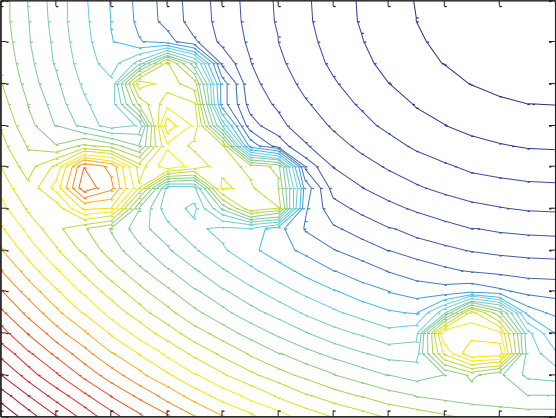
\includegraphics[width=.48\linewidth]{PotentialFieldTop}} \quad
    \subfloat[Perspective view]
    {\label{fig:PotentialFieldPerspective}
    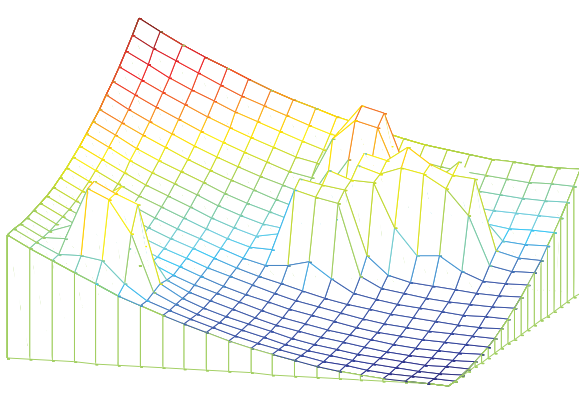
\includegraphics[width=.48\linewidth]{PotentialFieldPerspective}}
\caption[Example of potential field.]
{Example of potential field. The obstacles can be observed as a repulsive
component of the whole potential. Image credit: Liu \etal\cite{Liu2016}.}
\label{fig:potential-field}
\end{figure}

Once the potential function and the corresponding gradient have been
established, the solution path to a start-to-goal query can be incrementally
obtained by using the gradient descent, which is a widely-known algorithm in
solving optimization problems. Having $q_{start}$ as the initial configuration,
the algorithm iteratively calculates a new configuration by moving in the
direction opposite to the gradient until the gradient is zero. The pseudocode
for this method is presented in Algorithm~\ref{alg:Gradient-descent}.

\begin{algorithm}[htbp]
	\DontPrintSemicolon

	\KwIn{\\ 
	$q_{start}$: Start configuration.\\
	$\nabla U(q)$: Gradient of the potential field.}

 	\Begin{
 		$q(0) = q_{start}$\\
 		$i = 0$\\
 		\While{$\nabla U(q(i)) \neq 0$}{
 			$q(i + 1) = q(i) - \nabla U(q(i))$\\
 			$i = i + 1$
 		}
 	}
 \caption{Gradient Descent}
 \label{alg:Gradient-descent}
\end{algorithm}

However, the gradient descent algorithm using potential functions as explained
above does not guarantee finding or converging to a solution for a start-to-goal
query. This happens because it may reach a local minimum of $U(q)$ that may not
correspond to $q_{goal}$. To deal with such situations, Barraquand and Latombe
proposed the \ac{RPP}~\cite{Barraquand1990, Barraquand1991}, which is an
algorithm that makes use of the gradient descent together with random walks and
backtracking in order to avoid issues related to local minima. However, it is
important to note that \ac{RPP} effectiveness is highly dependent on parameter
tuning. Another important aspect to highlight is that \ac{RPP} was one of the
first methods to use a stochastic or random approach for path/motion planning;
algorithms with this characteristic will be discussed more in detail in
Section~\ref{sec:SamplingBasedAlg}.

% ----------------------- another section  ------------------------
\section{Roadmaps}
\label{sec:Roadmaps}

So far, the methods and algorithms presented above attempt to solve a single
start-to-goal query, which means they calculate a path that connects a start
configuration and a goal configuration. For doing so, they incrementally search
a path towards the goal while avoiding, at the same time, collisions with the
obstacles. Nonetheless, there are some applications in which the path/motion
planner is intended to solve more that one query. For those cases, it makes
sense to have a map that contains the information about all feasible routes, and
that can also be used more than once to solve multiple start-to-goal queries.
There are different alternatives to define a map that can be used for
path/motion planning, including topological, geometric, and grid-based
representations.

This section reviews methods that use a class of topological maps called
\textit{roadmaps}~\cite{Canny1993, Latombe1991}. A \ac{RM} is defined as
a subset of the \ac{C-Space} that results from the union of curves, in which any
$q_{start}$ and $q_{goal}$ contained in $\mathcal{C}_{free}$ can be connected by
a path that meets the following properties~\cite{Choset2005}:
\begin{inparaenum}[1)] \item \textbf{Accessibility} - there is a path from
$q_{start}\in\mathcal{C}_{free}$ to some $q'_{start}\in\mathcal{RM}$.
\item \textbf{Departability} - there is a path from some
$q'_{goal}\in\mathcal{RM}$ to $q_{goal}\in\mathcal{C}_{free}$.
\item \textbf{Connectivity} - there is a path in $\mathcal{RM}$ that
connects $q'_{start}$ and $q'_{goal}$.
\end{inparaenum}

\subsection{Visibility Graphs}

Visibility graphs are one of the alternatives in defining a roadmap. Assuming a
\ac{2D} \ac{C-Space} with polygonal obstacles, the set of the visibility graph
nodes ($v_i$) is composed of $q_{start}$, $q_{goal}$, and all the vertices of
the obstacles. Its edges, $e_{ij}$, are straight-line segments that can connect
any possible combination of two nodes $v_i$ and $v_j$, without colliding with
the obstacles ($e_{ij}\in\mathcal{C}_{free}$). Once the visibility graph is
fully defined, the solution path can be obtained by conducting any graph-based
search method, such as those explained in Section~\ref{sec:SearchBased}.
While Figure~\ref{fig:Visibility-Graph} depicts an example of a visibility graph
and a start-to-goal query solution over it, Algorithm~\ref{alg:Visibility-Graph}
presents the pseudocode to build a visibility graph.

\begin{figure}[htbp]
    \myfloatalign
    \subfloat[]
    {\label{fig:VisibilityGraph1}
    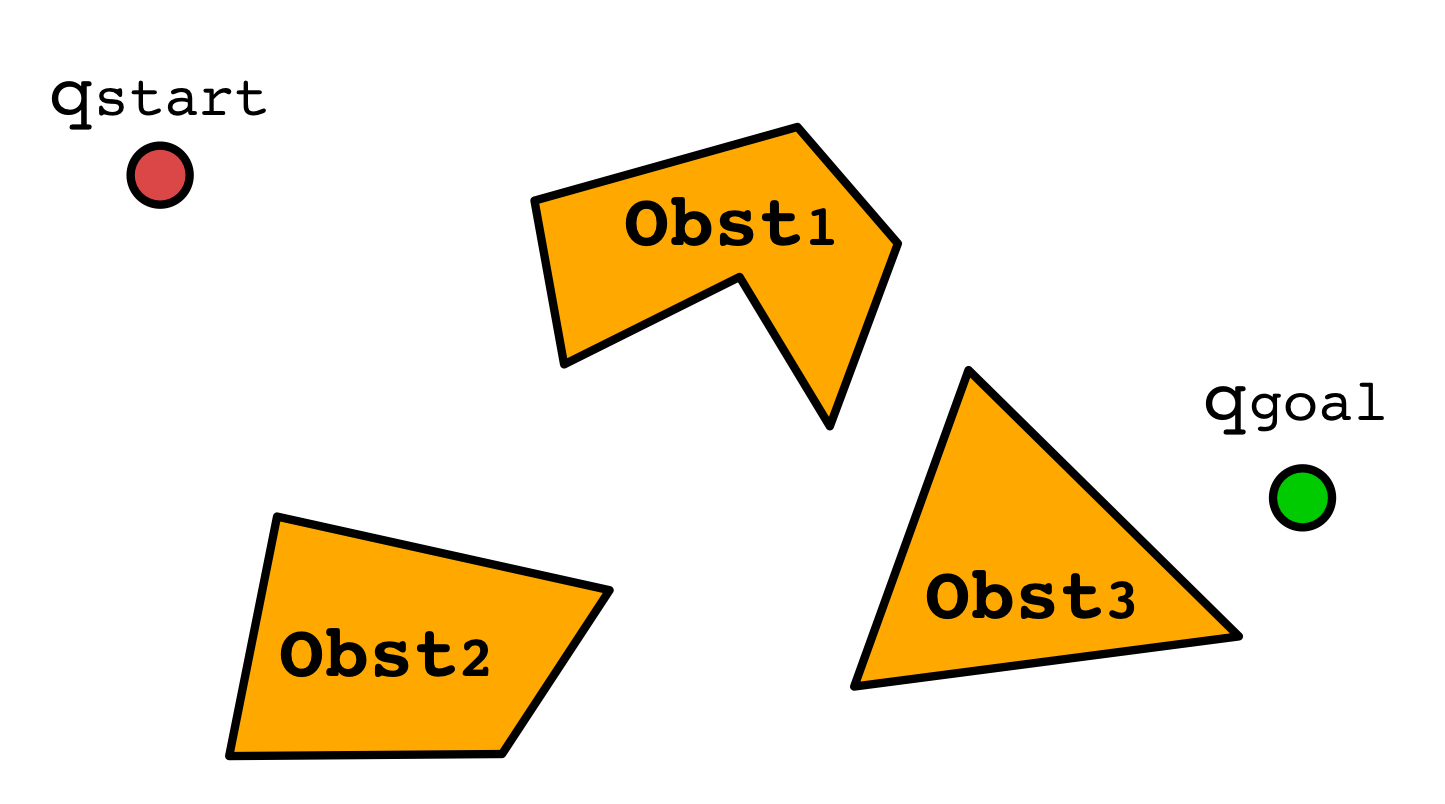
\includegraphics[width=.45\linewidth]{VisibilityGraph1}} \quad
    \subfloat[]
    {\label{fig:VisibilityGraph2}%
     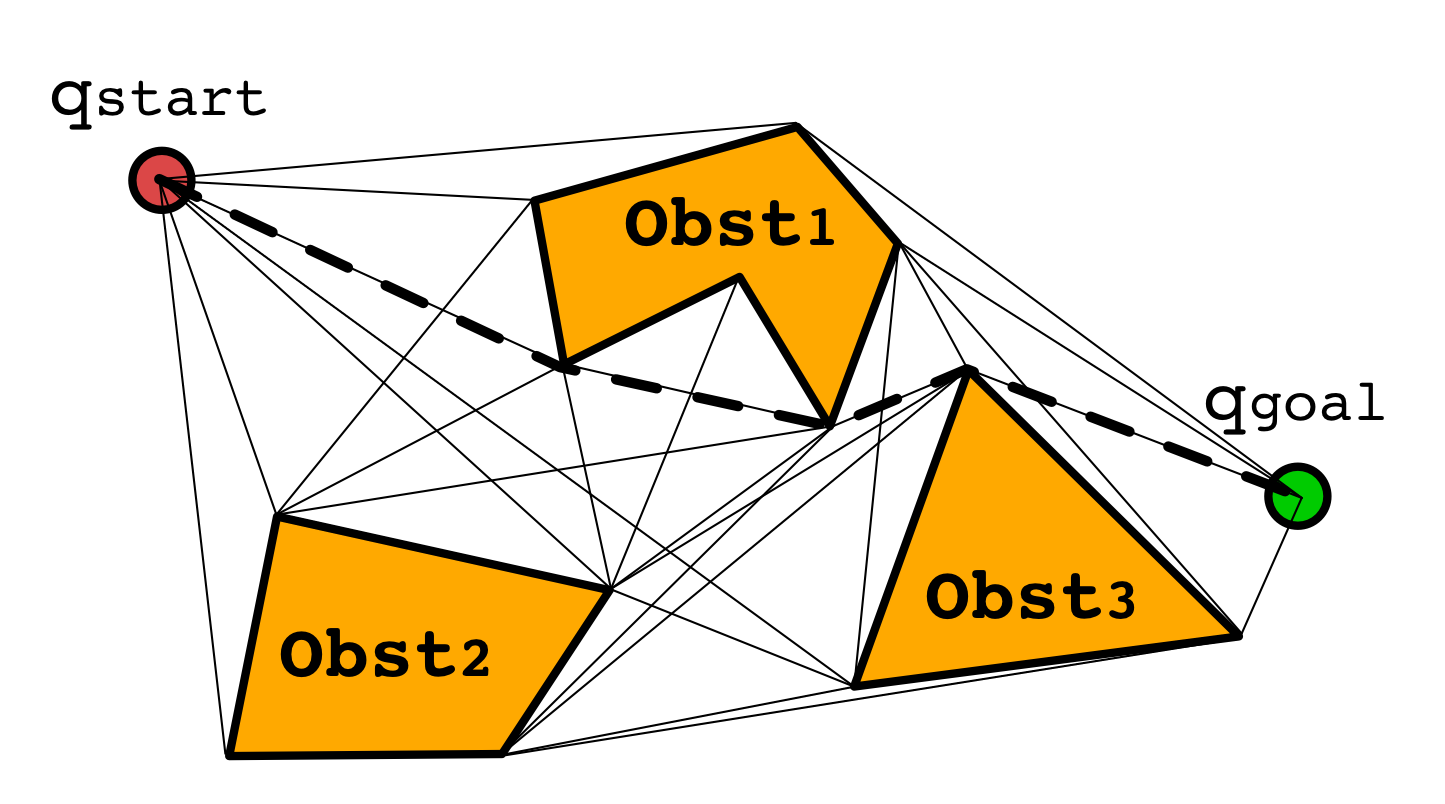
\includegraphics[width=.45\linewidth]{VisibilityGraph2}}
\caption[Example of a visibility graph.]
{Example of a visibility graph.
\protect \subref{fig:VisibilityGraph1} A 2D C-Space that contains polygonal
obstacles, a start configuration, and a goal configuration.
\protect \subref{fig:VisibilityGraph2} A roadmap is built by connecting any
possible combination of two vertices without colliding with the obstacles. The
start-to-goal query is solve using a graph search method.}
\label{fig:Visibility-Graph}
\end{figure}

\begin{algorithm}[htbp]
	\DontPrintSemicolon

	\SetKwFunction{addNodes}{addNodes}
	\SetKwFunction{getVertices}{getVertices}
	\SetKwFunction{getNumNodes}{getNumNodes}
	\SetKwFunction{findStraightLine}{findStraightLine}
	\SetKwFunction{isCollisionFree}{isCollisionFree}
	\SetKwFunction{addEdge}{addEdge}

	\KwIn{\\
	$q_{start}$: Start configuration.\\
	$q_{goal}$: Goal configuration.\\
	World: $n$ Obstacles.}
	
	\KwOut{\\
	Roadmap ($\mathcal{RM}$): Visibility Graph(VG) = $(V, E)$.}
	
	\Begin{
		$V=\{ \, \}$\;
		$E=\{ \, \}$\;
		\For{$ i=1:n$}{
	 		$V$.\addNodes{$Obst(i)$.\getVertices{}}\;
	 	}
	 	
	 	\For{$ i=1:$V$.\getNumNodes{}$}{
	 		\For{$ j=1:$V$.\getNumNodes{}$ and $j\neq i$}{
	 			$v_i\leftarrow$ $V(i)$\;
	 			$v_j\leftarrow$ $V(j)$\;
	 			$e_{ij}\leftarrow$ \findStraightLine{$v_i,v_j$}\;
	 			\If{\isCollisionFree{$e_{ij}$}}{
	 				$E$.\addEdge{$e_{ij}$}\;
 				}
	 		}
	 	}
 	}
 \caption{Visibility Graph}
 \label{alg:Visibility-Graph}
\end{algorithm}

\subsection{Generalized Voronoi Diagrams}

Another alternative to build a roadmap for path/motion planning is the \ac{GVD}.
The \ac{GVD} is defined for a set of points called \textit{sites}; given a
particular site, the set of points closest to it is called a \textit{Voronoi
region}. Finally, the Voronoi diagram is the set of points that are equidistant
to at least two sites~\cite{Aurenhammer1991}. In path/motion planning
applications, the \ac{GVD} defines the sets of points equidistant to at least
two obstacles. This means that the sites are the center of the obstacles to be
avoided, and the edges correspond to the possible channels that maximize the
distance to the obstacles~\cite{Choset2005}. Figure~\ref{fig:VoronoiDiagram}
displays an example of a planar \ac{GVD}.

\begin{figure}[htbp]
	\centering
	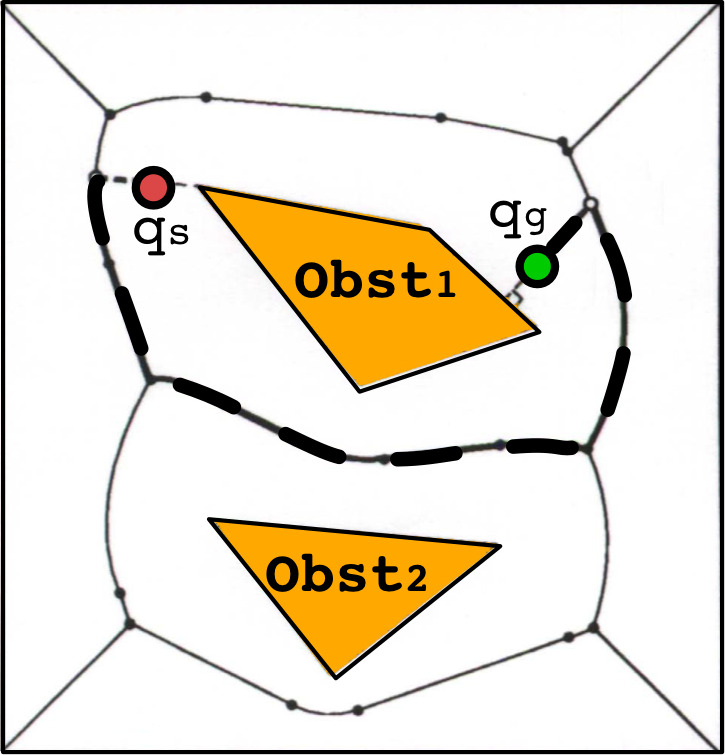
\includegraphics[width=.35\linewidth]{VoronoiDiagram}
\caption[Example of a voronoi diagram.]
{Example of a Voronoi diagram}	
\label{fig:VoronoiDiagram}
\end{figure}

% ----------------------- another section  ------------------------
% \section{Cell Decomposition}
% 
% Resolution completeness ?

%  \hl{Next, we consider a different type of representation of the free space
%  called an exact cell decomposition. These structures represent the free space by the union
% of simple regions called cells. The shared boundaries of cells often have a
% physical meaning such as a change in the closest obstacle or a change in line of
% sight to surrounding obstacles. Two cells are adjacent if they share a common
% boundary. An adjacency graph, as its name suggests, encodes the adjacency
% relationships of the cells, where a node corresponds to a cell and an edge
% connects nodes of adjacent cells.
% 
% Assuming the decomposition is computed, path planning with a cell decomposition
% is usually done in two steps: first, the planner determines the cells that
% contain the start and goal, respectively, and then the planner searches for a
% path within the adjacency graph. Note that the adjacency graph could serve as a
% roadmap of the free space as well. Therefore, mapping can be achieved by
% incrementally constructing the adjacency graph.
% 
% Cell decompositions, however, distinguish themselves from other methods in that
% they can be used to achieve coverage. A coverage path planner determines a path
% that passes an effector (e.g., a robot, a detector, etc.) over all points in a
% free space. Since each cell has a simple structure, each cell can be covered
% with simple motions such as back-and-forth farming maneuvers; once the robot
% visits each cell, coverage is achieved. In other words, coverage can be reduced
% to finding an exhaustive walk through the adjacency graph. Sensor-based coverage
% is achieved by simultaneously covering an unknown space and constructing its
% adjacency graph.
% 
% The most popular cell decomposition is the trapezoidal decomposition [356]. This
% decomposition relies heavily on the polygonal representation of the planar
% configuration space. A more general class of decompositions, which are termed
% Morse Decompositions [12], allow for representations of nonpolygonal and
% nonplanar spaces. Morse decompositions are based on ideas from Canny's roadmap
% work. We then consider a broader class of decompositions which includes those
% based on visibility constraints. One such decomposition serves as a basis for
% the pursuit/evasion problem which is introduced section 6.3. [Choset]
% 
% Cell decomposition refers to any method that partitions the free configuration
% space into a set of smaller cells [49]. Once the decompostion has been done, a
% connectivity graph can be built, where the cells are the nodes, and cells that
% share a common edge are connected in the graph. 
% 
% Cell decompositions are classified as either exact, semi-approximate, or
% approximate [49]. Within the cell decomposition methods, the major differences
% are generally based on how to generate the cells and what shape they should be.
% Pioneering work in this field was done by Acar and Choset. The Boustophedeon
% cell decomposition is first introduced in [48] and is based on previous work by
% Canny and Lin [43]. The cell decomposition is generated by determining critical
% points in the workspace where the connectivity of a slice, or 1-D line, of the
% free space changes as it is swept across the workspace. This is expanded in [1,
% 2] to include a method in which critical points can be detected online and the
% decomposition is referred to as a Morse decomposition. The connectivity of the
% cells is represented by the Reeb graph. In [3], the approach is applied to a
% terrestrial demining task where the robot is able to detect and exploit the
% pattern of the mines to search more efficiently. In [4], the algorithm is
% extended to apply to a robot whose sensor swath is larger than the platform
% footprint. In this approach, two heuristics are combined: one for coverage of
% wide open spaces based on Boustrophedon search, and one for constricted areas
% which is based on the GVD. 
% 
% Once the cell decomposition is made, a graph is generated where each cell
% represents a node in the tree and adjacent cells are connected with an edge. As
% mentioned, this type of decomposition is most useful for achieving coverage, but
% start-to-goal planning can be done by reducing each cell to one or a few points.
% In Fig. 2.10 each cell has been reduced to its centroid. The centroids of cells
% in the figure are denote by black dots. The blue lines represent the critical
% slices. Note that every critical slice is tangent to an obstacle but cannot
% penetrate an obstacle. As per the earlier figures, the obstacles are shown in
% red. The path found by connecting centroids is shown as the yellow line. Note
% that in this simplistic case, a suboptimal path is generated because of the
% reduction of the cells to only their centroids. [Paull13]}

% \begin{figure}[htbp]
% 	\centering
% 	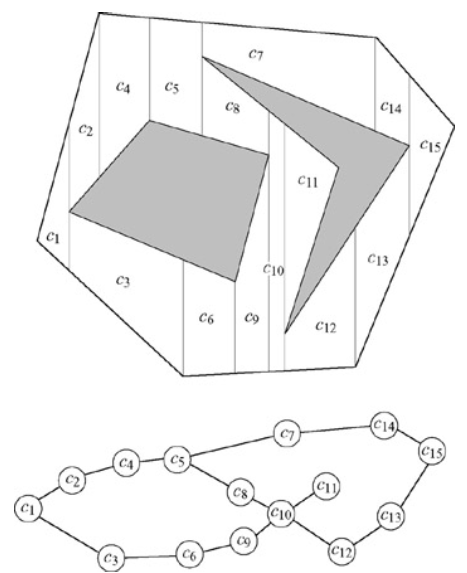
\includegraphics[width=.45\linewidth]{Cell-Decomposition} \quad
% 	\caption{\hl{Cell-Decomposition}}
% 	\label{fig:Cell-Decomposition}
% \end{figure}

% ----------------------- another section  ------------------------
\section{Sampling-based Algorithms}
\label{sec:SamplingBasedAlg}

Some of the methods presented in previous sections, such as potential fields,
roadmaps, and cell decomposition, require an explicit representation of
$\mathcal{C}_{free}$ in order to find a collision-free path from a start
configuration to a goal configuration. Nonetheless, there are some situations in
which building such a representation is not possible or is computationally
intractable, for instance when dealing with high-dimensional configuration
spaces. For those cases, sampling-based methods have been demonstrated to be
effective.

Firstly developed during the 90's, \textit{sampling-based algorithms} are an
alternative approach that aims to create a sampled (discrete) representation of
\ac{C-Space} that captures the connectivity of the regions of
$\mathcal{C}_{free}$. These methods exploit the fact that, while explicitly
building $\mathcal{C}_{free}$ is expensive, checking a given configuration for
collisions can be done quickly. To build such a discrete representation, they
firstly generate random samples $q_{r_i}$ from \ac{C-Space}, which are checked
for collision in order to ensure that $q_{r_i} \in \mathcal{C}_{free}$.
Secondly, they interconnect the random and collision-free configurations, thus
establishing different routes (paths) to solve single or multiple start-to-goal
queries. This two-stage (sampling and connecting) approach that uses a collision
checking routine to validate samples, also allows generalizing the path/motion
planning problem. This is done by separating the algorithm from the specific
geometric representation of the environment.

However, there is one important characteristic to be considered when using
sampling-based algorithms. Contrary to the methods mentioned previously,
sampling-based algorithms weaken the completeness guarantee, which means that
they are not capable of notifying if a solution exists.
Nonetheless, given that many of these methods are based on random sampling,
which is dense with probability one~\cite{LaValle2006}, this also implies that
with enough points (samples), if a solution exists then the probability of
finding it converges to one.
In other words, if the algorithm runs for a sufficient amount of time, it will
find a solution if there is one. This property is called \textit{probabilistic
completeness}~\cite{Kavraki1996,Barraquand1997,Kavraki1998}.

These characteristics have led sampling-based algorithms to be considered the
state-of-the-art approach for solving various path/motion planning problems.
Albeit there are several methods and variants used nowadays, it is possible to
identify those that, at the time, were pioneers and the most relevant ones. This
section presents such methods and classifies them according to their capability
to solve single or multiple start-to-goal queries.

\subsection{Multiple-query Methods}

As it was explained in Section~\ref{sec:Roadmaps}, roadmaps are data structures
that contain all feasible routes that can be used more than once to solve
multiple start-to-goal queries. Likewise, there is a sampling-based method
called \ac{PRM} that creates a graph attempting to represent the connectivity of
$\mathcal{C}_{free}$. \ac{PRM} was developed simultaneously at
Stanford~\cite{Kavraki1994,Kavraki1994a} and Utrecht~\cite{Overmars1994}, and
was jointly presented in 1996~\cite{Kavraki1996}.

Nowadays, \ac{PRM} is one of the most representative sampling-based algorithms.
It is mainly composed of a \textit{preprocessing phase} and a \textit{query
phase}. During the first phase, the algorithm builds a roadmap, or undirected
graph $G=(V,E)$. The set of nodes $(V)$ contains $n$ collision-free samples
$q_{r_i}$ (\ie $q_{r_i} \in \mathcal{C}_{free}$) that are randomly obtained from
an uniform distribution\footnote{Uniform distribution is the basic form to
obtain the random samples, at least in the basic version of the algorithm.
Other distributions have been used in some extensions of the original method.}.
The set of edges $(E)$ corresponds to the collision-free paths from each node
$q_{r_i}$ to its $k$ closest nodes $q_{r_j}$; the connecting paths are
calculated by a local planner that checks them for collisions.
Algorithm~\ref{alg:PRM-Preprocessing-Phase} presents the pseudocode for the
\textit{preprocessing phase}.

\begin{algorithm}[htbp]
	\DontPrintSemicolon

	\SetKwFunction{generateRandomConf}{generateRandomConf}
	\SetKwFunction{addNode}{addNode}
	\SetKwFunction{getNodes}{getNodes}
	\SetKwFunction{getClosestNodes}{getClosestNodes}
	\SetKwFunction{findPath}{findPath}
	\SetKwFunction{isCollisionFree}{isCollisionFree}
	\SetKwFunction{addEdge}{addEdge}

	\KwIn{\\
	$n$: Number of nodes of the roadmap.\\
	$k$: Number of closest nodes to attempt connection.\\
	$\mathcal{C}$: \ac{C-Space}}
	
	\KwOut{\\
	Probabilistic roadmap ($PRM$): G = $(V, E)$.}
	
	\Begin{
		$V=\{ \, \}$\;
		$E=\{ \, \}$\;
		\While{$|V|< n$}{
			$q_{rand}=\mathcal{C}.$\generateRandomConf{}\;
			\If{$\mathcal{C}.$\isCollisionFree{$q_{rand}$}}{
	 			$V$.\addNode{$q_{rand}$}\;
 			}
	 	}
	 	
	 	\For{$q_{r_i}\in V$.\getNodes{}}{
	 		\For{$q_{r_j}\in \,\mathcal{C}.$\getClosestNodes{$q_{r_i}, k$}}{
 	 			$e_{ij}\leftarrow$ \findPath{$q_{r_i},q_{r_j}$}\;
	 			\If{$\mathcal{C}.$\isCollisionFree{$e_{ij}$}}{
	 				$E.$\addEdge{$e_{ij}$}\;
 				}
 	 		}
	 	}
 	}
 \caption{PRM, preprocessing phase}
 \label{alg:PRM-Preprocessing-Phase}
\end{algorithm}

Once the roadmap (graph) has been built, the \textit{query phase} attempts to
find a collision-free path between the provided $q_{start}$ and $q_{goal}$. To
do so, \ac{PRM} tries to connect $q_{start}$ and $q_{goal}$ to their $k$ closest
nodes in the graph $G$. If the connections are successful, a search-based method
(\eg A*, Dijkstra, etc.) attempts to find the shortest path over the graph. If
the connections for $q_{start}$ and $q_{goal}$ to the graph are not possible, or
if the search-based algorithm fails to find a solution path for the query, it
does not necessarily mean that a solution does not exist. As explained above,
most sampling-based methods, including \ac{PRM}, are probabilistic complete,
which means that more time may be required to find a solution, if there is one.
In this case, it would imply that the number of nodes $n$ have to be increased,
as that will generate a more dense probabilistic roadmap.

An important number of variants and extensions have been proposed to deal with
different situations in which the originally proposed \ac{PRM} may
fail~\cite{Choset2005},~\cite{LaValle2006}. A typical example includes a
workspace that creates a \ac{C-Space} with narrow passages. In such a case, a
common approach would be oversampling the regions of interest (\eg narrow
passages), thus increasing the probability of finding a solution path. Other
extensions that have served as a base for the work developed throughout this
thesis, will be discussed in Section~\ref{sec:ExtensionsApplications}.
Finally, Figure~\ref{fig:PRM} depicts \ac{PRM} solving a start-to-goal query in
a \ac{2D} scenario for a point-like robot.

\begin{figure}[htbp]
	\centering
	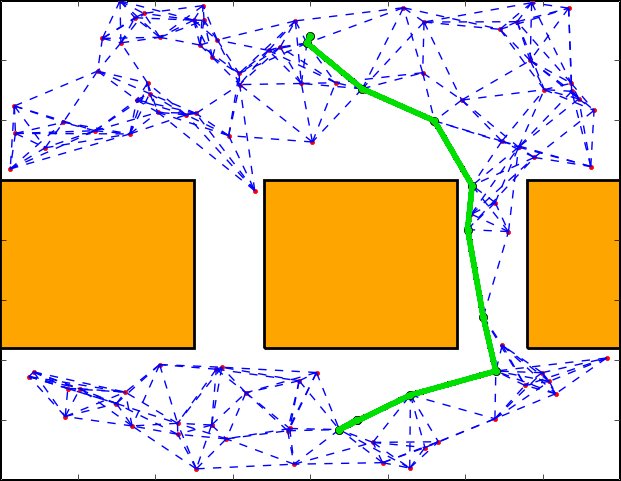
\includegraphics[width=.55\linewidth]{PRM} \quad
\caption[Example of a probabilistic roadmap (PRM) used to solve a start-to-goal
query.]
{Example of a probabilistic roadmap (PRM) used to solve a start-to-goal query.
The PRM was built with $100$ random samples, which were attempted to connect to
their $6$ nearest neighbors.}
\label{fig:PRM}
\end{figure}

\subsection{Single-query Methods}

There is another group of sampling-based algorithms that is devoted to solving a
single start-to-goal query. Such methods conduct an incremental search, which in
most cases is achieved by expanding a tree of randomly sampled configurations.
The search is generally biased to finding a solution path for one particular
start-to-goal query, rather than attempting to completely represent the
connectivity of $\mathcal{C}_{free}$. These methods are \textit{unidirectional}
when a single tree is expanded from $q_{start}$ until reaching $q_{goal}$ or
vice versa. Or, they are \textit{bidirectional} if two trees are expanded, one
from $q_{start}$ and other from $q_{goal}$, until both trees meet at a common
point. Choosing $q_{start}$ or $q_{goal}$ as the tree's root depends on the
specific problem and scenario, since there can be situations in which expanding
from the goal is easier (less constrained) that doing it from the start
configuration. There are different sampling-based single-query methods, however,
this section presents a brief review of those considered the most relevant.

\subsubsection{Randomized Path Planner (RPP)}

Section~\ref{sec:PotenFields} presented an approach for guiding a robot from its
current position towards the goal position, by following the negative gradient
of an artificial potential field. As mentioned there, one of the main
disadvantages of this approach is that the vehicle can get trapped in a local
minimum that may not correspond to the specified goal. In order to deal with
such situations, Barraquand and Latombe proposed in 1990 the randomized path
planner (\ac{RPP})~\cite{Barraquand1990,Barraquand1991}, which uses the strategy
of potential fields, but also incorporates random walks to escape local minima.
\ac{RPP} is commonly acknowledged as the first randomized algorithm. Albeit
\ac{RPP} has proved to be successful in many applications, it may fail when
coping with narrow passages.

\subsubsection{The Ariadne's Clew Algorithm (ACA)}

Presented in 1993, \ac{ACA} builds a tree from $q_{start}$ by interleaving the
\textit{exploration} of the \ac{C-Space} and the \textit{search} of a connection
between the tree and $q_{goal}$~\cite{Bessiere1993,Mazer1998}. During the
exploration, the algorithm places a random collision-free configuration as far
as possible from the others, therefore guaranteeing resolution completeness. New
configurations are selected by using genetic optimization methods. These
correspond to those from which a connection to $q_{goal}$ is attempted. The main
drawback of this approach is that the exploration of the \ac{C-Space} is
computationally expensive and also requires some parameter tuning.

\subsubsection{Expansive-Spaces Tree (EST)}

Proposed by David Hsu \etal in 1997,
\ac{EST}~\cite{Hsu1997,Hsu1999,Hsu2000,Hsu2002} is a single-query method that
incrementally builds a tree over the \ac{C-Space} by interleaving its
\textit{construction} and \textit{expansion}. In contrast to what occurs with
\ac{PRM} that computes a roadmap attempting to represent the whole
$\mathcal{C}_{free}$, \ac{EST} tries to sample the region of $\mathcal{C}$ that
is relevant in order to solve the specific start-to-goal query. To do so, during
the \textit{construction} phase the algorithm selects the node $q$ to be
extended in a way that prioritizes less explored regions, and then it randomly
samples a configuration $q_{rand}$ around $q$. Then, using a local planner,
\ac{EST} calculates the path that connects $q$ and $q_{rand}$. In case that both
$q_{rand}$ and the calculated path are proved collision-free, they will be added
to the tree, thus \textit{expanding} it.

\subsubsection{Rapidly-exploring Random Tree (RRT)}
\label{sec:RRT}

Within the group of sampling-based single-query algorithms, there is one method
that is considered the state-of-the-art, which has been extended, modified and
applied to a wide range of applications. This method is known as \ac{RRT} and it
was firstly presented by Steven LaValle in 1998~\cite{LaValle1998}.
\ac{RRT} is a tree-based algorithm that has different properties such as rapid
exploration of the \ac{C-Space}, probabilistic completeness, ease of
implementation, just to mention some. In 1999, LaValle and Kuffner formally
presented the \ac{RRT} as a path/motion planning method capable of dealing with
both geometric and motion constraints. They also proposed a greedy approach to
decrease the time required to find a solution by interleaving a random growing
of the tree with a biased growing towards the
goal~\cite{LaValle1999,LaValle2000,LaValle2001}. They later proposed a
bidirectional version called RRT-Connect that extends the basic concept by
constructing two \acp{RRT} towards each other~\cite{Kuffner2000}.

Similar to \ac{ACA} and \ac{EST}, the basic \ac{RRT} is mainly composed of two
main procedures, \textit{sample} and \textit{extend}.
Algorithm~\ref{alg:SampleRRT} presents the first of them, where the tree is
incrementally built until a stop condition occurs; such a condition can either
be finding a feasible path that reaches the goal close enough, or that a maximum
number of iterations has been completed. In each iteration, the \ac{RRT}
attempts to extend the tree towards a randomly sampled configuration $q_{rand}$.
For doing so, the second procedure described in Algorithm~\ref{alg:ExtendRRT}
finds $q_{near}$, which is the nearest configuration to $q_{rand}$ in the tree
(line~\ref{alg_line:findNearestGeom}).
Then, a local planner calculates a path of length $\delta$ from $q_{near}$
towards $q_{rand}$ (line~\ref{alg_line:ExtendRRTGeom}); if the path is proved
collision-free, the algorithm generates a new configuration $q_{new}$, which
together with the calculated path are added to the tree
(lines~\ref{alg_line:addNodeGeom}-\ref{alg_line:addEdgeGeom}). A typical growth
process of an \ac{RRT} can be clearly observed in
Figure~\ref{fig:RRT-Expansion}, where no goal has been specified and the tree
attempts to explore uniformly the \ac{C-Space}.
Figure~\ref{fig:RRT-Solve-Query} depicts the \ac{RRT} solving a start-to-goal
query.

\begin{algorithm}[htbp]
	\DontPrintSemicolon

	\SetKwFunction{stopCondition}{stopCondition}
	\SetKwFunction{initTree}{initTree}
	\SetKwFunction{generateRandomConf}{generateRandomConf}
	\SetKwFunction{extendRRT}{extendRRT}
	\SetKwFunction{addNode}{addNode}
	
	\KwIn{\\ 
	$q_{start}:$ Start configuration. \\ 
	$q_{goal}:$ Goal configuration.\\
	$\mathcal{C}$: \ac{C-Space}.}
	
 	\KwOut{\\ 
 	Rapidly-exploring Random Tree ($RRT$): T = $(V, E)$.}
 	
	\Begin{
		$V=\{ \, \}$\;
		$E=\{ \, \}$\;
		$V$.\addNode{$q_{start}$}\;
		\While{not \stopCondition{$T,goal$}}{
			$q_{rand}=\mathcal{C}.$\generateRandomConf{}\;
	 		\extendRRT{$T,q_{rand}$}\;
		}
	}
\caption{sampleRRT}
\label{alg:SampleRRT}
\end{algorithm}

\begin{algorithm}[htbp]
\DontPrintSemicolon

	\SetKwFunction{calcNewConf}{calcNewConf}
	\SetKwFunction{findNearestNeighbor}{findNearestNeighbor}
	\SetKwFunction{addNewNode}{addNewNode}
	\SetKwFunction{addNewEdge}{addNewEdge}
	
	\KwIn{\\ 
	$T$: an RRT.\\ 
	$q_{rand}$: configuration towards which RRT will be extended.\\
 	$\mathcal{C}$: \ac{C-Space}.}
	\KwOut{\\ Result after attempting to extend.}
	\Begin{
	 	$q_{near}\leftarrow T.$\findNearestNeighbor{$q_{rand}$}\;\label{alg_line:findNearestGeom}
	 	$q_{new}, collision\leftarrow$\calcNewConf{$q_{near},q_{rand},\delta$}\;\label{alg_line:ExtendRRTGeom}
	 	\If{$collision = FALSE$} { 
	 		V.\addNewNode{$q_{new}$}\;\label{alg_line:addNodeGeom}
	 		E.\addNewEdge{$q_{near},q_{new}$}\;\label{alg_line:addEdgeGeom}
	 		\KwRet{$\text{ADVANCED}$}\label{lin_alg:Adva}
  		}
  		\Else{
  			\KwRet{$\text{TRAPPED}$}\label{lin_alg:Trapp}
  		}
 	}
\caption{extendRRT}
\label{alg:ExtendRRT}
\end{algorithm}

\begin{figure}[htbp]
    \myfloatalign
    \subfloat[RRT expansion]
    {\label{fig:RRT-Expansion}
    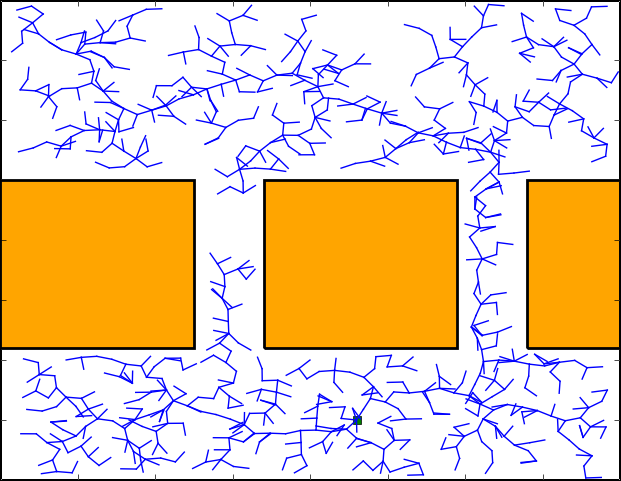
\includegraphics[width=.45\linewidth]{RRT-Expansion}} \quad
    \subfloat[RRT solving a query]
    {\label{fig:RRT-Solve-Query}%
     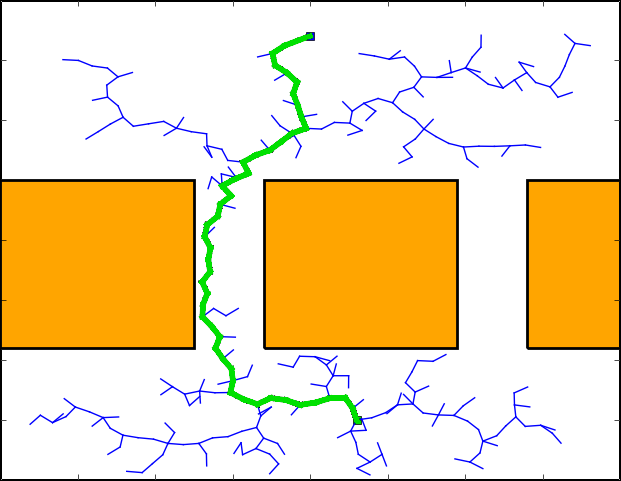
\includegraphics[width=.45\linewidth]{RRT-Solve-Query}}
\caption[Example of a rapidly-exploring random tree (RRT).]
{Example of a rapidly-exploring random tree (RRT) in a 2D workspace. 
\protect \subref{fig:RRT-Expansion} The uniform and rapid exploration of the
C-Space is one of the main characteristics.
\protect \subref{fig:RRT-Solve-Query} The expansion of the tree stops once a
solution has been found.}
\label{fig:RRT}
\end{figure}

\subsection{Optimal Planning}
\label{sec:SamplOptimalPlan}

At least in their original formulation, sampling-based algorithms do not
guarantee that the calculated path is optimal with respect to a specified cost
function. However, more recent contributions have attempted to cope with this
situation. In 2010, Jaillet \etal presented the \ac{T-RRT}, which calculates a
low-cost path that follows valleys and saddle points in a costmap established
over the \ac{C-Space}~\cite{Jaillet2010}. To achieve this, it verifies the
quality of the path by using the minimal work criterion. Its key principle is
that positive variations of the cost function can be seen as forces acting
against motion, and thus producing mechanical work. Contrasted to a standard
\ac{RRT} implementation, an additional transition validation is performed, which
accepts or rejects new potential configurations before adding them into the
solution tree.

Nonetheless, the state-of-the-art sampling-based method for calculating optimal
paths is the \ac{RRT*}. In 2010, Karaman and Frazzoli firstly introduced the
\ac{RRT*} and its concept of asymptotic optimality. This property states that
the total cost of the solution, measured by a user-defined function, decreases
as the number of samples increases~\cite{Karaman2010a}. In this approach, new
configurations are connected to the closest and best configuration, \ie the one
that guarantees a minimum cost. Furthermore, an additional step of sample
reconnection allows improving costs to surrounding configurations (see
Algorithm~\ref{alg:ExtendRRTstar}). This concept was later extended by the same
authors to the \ac{PRM} in~\cite{Karaman2011}, where they formally presented the
\ac{RRT*} and PRM*. Similar extensions have been done to other RRT-based
algorithms as \ac{T-RRT} and its respective T-RRT* version~\cite{Devaurs2016}. A
typical growth process of an \ac{RRT*} can be clearly observed in
Fig.~\ref{fig:RRTstar}.

\begin{algorithm}[htbp]
    \DontPrintSemicolon

	\SetKwFunction{buildRRT}{buildRRT}
	\SetKwFunction{calculatePath}{calculatePath}
	\SetKwFunction{findNearestNeighbor}{findNearestNeighbor}
	\SetKwFunction{addNewNode}{addNewNode}
	\SetKwFunction{addNewEdge}{addNewEdge}
	\SetKwFunction{findNearestNeighbors}{findNearestNeighbors}
	\SetKwFunction{findMinCost}{findMinCost}
	\SetKwFunction{reconnectNearNeighbors}{reconnectNearNeighbors}
	\SetKwFunction{findInput}{findInput}
	
	\KwIn{\\
	$T$: tree of collision-free configurations.\\
	$q_{rand}$: state towards which the tree will be extended.\\
 	$\mathcal{C}$: C-Space.}
	\KwOut{\\ 
	Result after attempting to extend.}
	\Begin{
	 	$q_{near}\leftarrow T.$\findNearestNeighbor{$q_{rand}$}\;
	 	$q_{new}, collision\leftarrow$\calcNewConf{$q_{near},q_{rand},\delta$}\;%label{alg_line:ExtendRRTGeom}
	 	\If{$collision = FALSE$} {
  			\addNewNode{$T,q_{new}$}\;
  			$Q_{near}\leftarrow$\findNearestNeighbors{$T,q_{new}$}\;\label{lin_alg:FindNearNeighbors}
  			$q_{min\_cost}\leftarrow$\findMinCost{$T,Q_{near},q_{new}$}\;\label{lin_alg:FindMinCost}
  			\addNewEdge{$T,q_{min\_cost},q_{new}$}\;\label{lin_alg:AddNewEdge}
  			\reconnectNearNeighbors{$T,Q_{near},q_{new}$}\;\label{lin_alg:ReconnNearNeighbors}
  			\KwRet{$\text{ADVANCED}$}\;%\label{lin_alg:Adva}
  		}
  		\Else{
  			\KwRet{$\text{TRAPPED}$}\;%\label{lin_alg:Trapp}
  		}
 	}
\caption[.]{extendRRT*}
\label{alg:ExtendRRTstar}
\end{algorithm}


\begin{figure}[htbp]
    \myfloatalign
    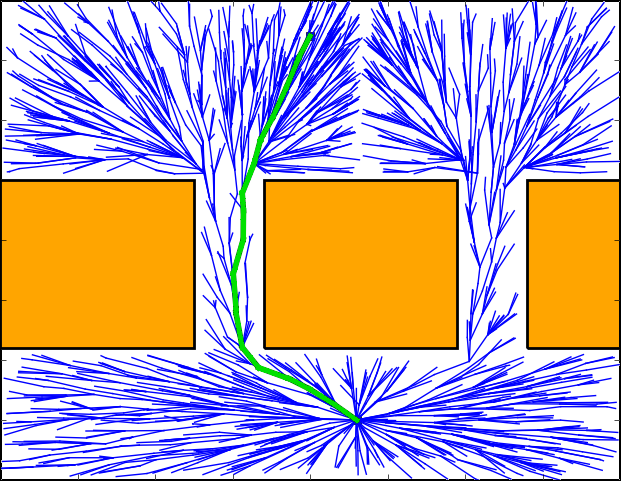
\includegraphics[width=.55\linewidth]{RRTStar-Expansion}
\caption[Example of an asymptotic optimal rapidly-exploring random tree (RRT*).]
{Example of an asymptotic optimal rapidly-exploring random tree (RRT*) in a 2D
workspace. The RRT* preserves the uniform and rapid exploration of the C-Space
as the standard RRT; however, it can be observed how the additional reconnection
step reshapes the tree branches. The expansion of the tree does not stop once a
solution has been found. Instead, it keeps improving the solution until either a
maximum number of iterations or a maximum time has been reached.}
\label{fig:RRTstar}
\end{figure}

% \begin{algorithm}[htbp]
% 	\dontprintsemicolon
% 	\SetKwFunction{findNearestNeighbor}{findNearestNeighbor}
% 	\SetKwFunction{findInput}{findInput}
% 	\SetKwFunction{calcNewConf}{calcNewConf}
% 	\SetKwFunction{addNewNode}{addNewNode}
% 	\SetKwFunction{addNewEdge}{addNewEdge}
% 	\SetKwFunction{findNearestNeighbors}{findNearestNeighbors}
% 	\SetKwFunction{findMinCost}{findMinCost}
% 	\SetKwFunction{reconnectNearNeighbors}{reconnectNearNeighbors}
% 	
%  	\KwIn{\\ $T$: configurations tree (RRT).\\
%  			  $q_{rand}$: state which RRT will be attempted to extend to.\\}
%  	\KwOut{\\ Result after attempting extension. \\
%  			  $q_{new}$: New configuration if succeeded.}
%  	
%  	\Begin{
%   		$q_{near}\leftarrow$\findNearestNeighbor{$T,q_{rand}$}\;
%   		$u_{near\_rand}\leftarrow$\findInput{$T,q_{near},q_{rand}$}\;\label{lin_alg:FindInputRRT}
%   		$q_{new}, collision\leftarrow$\calcNewConf{$q_{near},u_{near\_rand}$}\;
%   		\If{{\bf not} $collision$} { 
%   			\addNewNode{$T,q_{new}$}\;
%   			$Q_{near}\leftarrow$\findNearestNeighbors{$T,q_{new}$}\;\label{lin_alg:FindNearNeighbors}
%   			$q_{min\_cost}\leftarrow$\findMinCost{$T,Q_{near},q_{new}$}\;\label{lin_alg:FindMinCost}
%   			\addNewEdge{$T,q_{min\_cost},q_{new}$}\;\label{lin_alg:AddNewEdge}
%   			\reconnectNearNeighbors{$T,Q_{near},q_{new}$}\;\label{lin_alg:ReconnNearNeighbors}
%   			\KwRet{$\text{ADVANCED}$}\label{lin_alg:Adva}
%   		}
%   		\Else{
%   			\KwRet{$\text{TRAPPED}$}\label{lin_alg:Trapp}
%   		}
%  }
%  \caption{extendRRT$(T,q_{rand})$}
%  \label{alg:ExtendRRT}
% \end{algorithm}

% \cite{Ferguson2006}
% \cite{Li2002}
% 
% \cite{Bruce2002}, \cite{Stentz1995}, \cite{Carsten2006}, \cite{Leven2002},
% \cite{Barraquand1990}, \cite{Shvalb2013}, \cite{Valencia2012}, \cite{Mora2013},
% \cite{Karaman2011}, \cite{Salzman2013}, \cite{Muller2011}, \cite{Zhu2013},
% \cite{Poppinga2011}, \cite{Li2010}, \cite{Ardiyanto2011}, \cite{Dobson2013},
% \cite{Sucan2008}, \cite{Howard2014}, \cite{Ladd2005}, \cite{Ghosh2008},
% \cite{Xue2009}, \cite{Dolgov2010}, \cite{Smith2010}, \cite{Likhachev2009},
% \cite{Dolgov2008}, \cite{Aoude2013}, \cite{Maki2007}, \cite{Vannoy2008},
% \cite{Quinlan1994}, \cite{Kuwata2009}, \cite{Karaman2011}, \cite{Tsianos2007},
% \cite{Masehian2008}, \cite{Dobson2012,Dobson2014}, \cite{Thrun2006},
% \cite{Kewlani2009}, \cite{Kim2009}
% 
%  
% 
% However, one of them, a graph-based approach known as
% \textit{\ac{RRG}}~\cite{Karaman2009}, attempts to minimize a cost function.
% That method has been modified in order to guarantee an asymptotic optimality as
% is known as
% \textit{\ac{RRT*}}~\cite{Karaman2010,Karaman2010,Karaman2011,Karaman2011}

% ----------------------- another section  ------------------------
\section{Extensions and Applications}
\label{sec:ExtensionsApplications}

Most of the aforementioned methods have been widely used in real-world
applications not only with manipulator arms, but also with different aerial,
terrestrial and aquatic robotic systems. For doing so, some of these methods
have been extended and adapted according to the specific applications'
requirements. Considering the problem and objectives stated for this thesis in
Chapter~\ref{ch:introduction}, this section presents a brief review of the most
relevant extensions and applications of path/motion planning algorithms, which
have permitted conducting autonomous missions under both motion and online
computation constraints.

% ----------------------- subsection  ------------------------
\subsection{Path/Motion Planning under Motion Constraints}
\label{sec:motion_constraints_review}

As explained in Section~\ref{sec:PlannUnderConst}, planning under motion
(differential) constraints has to do with considering the limits of the feasible
system's maneuvers. These are described by a set of differential equations,
generally expressed as $\dot{q}=f\left(q,u\right)$ (where $q$ and $\dot{q}$ are
the system state and its first derivative, respectively, and $u$ is the control
input). A large body of research has been dedicated to the development and
improvement of different approaches attempting to solve planning problems that
include this kind of constraints.

When Donald \etal formally introduced the problem of kinodynamic motion
planning\footnote{Kinodynamic motion planning alternatively refers to motion
planning under motion or differential constraints.}, they proposed the use of
dynamic programming to find the shortest path in a directed graph using
\ac{DFS}. In this case, the graph represents a discretization of
$\mathcal{C}_{free}$; the edges correspond to trajectory segments obtained after
applying an acceleration $a$ (bounded according to the system's capabilities)
for a period of time $\tau$ (determined by the algorithm)~\cite{Donald1993}.

Other variants of grid-based methods, such as A*, have been also used with
similar strategies for discretizing $\mathcal{C}_{free}$. In terrestrial
vehicles, for example, the most remarkable contributions were a result of the
DARPA Grand Challenge~\cite{Thrun2006}\footnote{The DARPA Grand Challenge is a
competition of autonomous vehicles, funded by the Defense Advanced Research
Projects Agency (DARPA).}. In one of those works, Likhachev and Ferguson used a
multi-resolution lattice state space (a $\mathcal{C}_{free}$ discretization),
where states represent configurations, and connections between them represent
feasible paths (\ie those that consider kinematic constraints).
Then, one A* variant (called AD*) would find paths over the
lattice~\cite{Likhachev2009}. Similarly, Dolgov \etal presented an approach in
which $\mathcal{C}_{free}$ is also discretized and paths are found by running
another A* variant (Hybrid-State A*). This is guided by two heuristics, one that
considers the vehicle's non-holonomic constraints and a second one that computes
the Euclidean distance. This approach also connects the states (configurations)
by restricting the control inputs according to the feasible (doable) maneuvers
of a car-like system, which are expressed by non-holonomic (kinematic)
constraints~\cite{Dolgov2008,Dolgov2010}.

In all these grid-based approaches, the main drawback is given by the
$\mathcal{C}_{free}$ discretization, which establishes a finite set of possible
maneuvers, thus limiting the number of possible solution paths. As occurs with
geometric path planning approaches, the availability of a solution depends on
the grid resolution and, in this case, on the number of maneuvers considered
according to the motion constraints.

In what concerns sampling-based methods, \ac{EST} and \ac{RRT} were initially
conceived to cope with motion constraints~\cite{Hsu2002,LaValle2001}. In their
original versions, the differential equation of motion is used to generate new
nodes (states) during the \textit{expansion} of the tree (\eg in
Algorithm~\ref{alg:ExtendRRT}, line 3)\footnote{While tree and graph nodes are
generally referred to as configurations in geometric path planning, in
kinodynamic motion planning they are commonly called states. However, this
latter term has been indistinctly used by some authors to refer to them in
either case.}. Figure~\ref{fig:PlannConst} depicts two sampling-based
algorithms: \ac{RRT*} and \ac{RRT} in the process of solving a start-to-goal
query in a \ac{2D} workspace under both geometric and motion constraints.

\begin{figure}[htbp] \myfloatalign
	\subfloat[Geometric Constraints] {\label{fig:PlannGeomConstr_}
    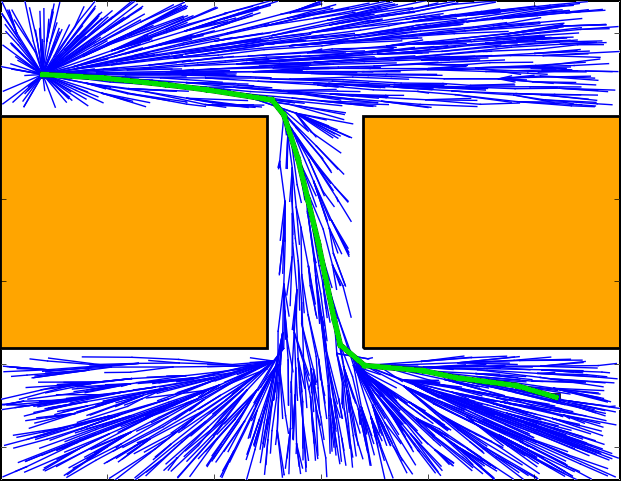
\includegraphics[width=.4\linewidth]{PlannGeomConstr}} \quad
    \subfloat[Differential Constraints] {\label{fig:PlannDiffConstr}
    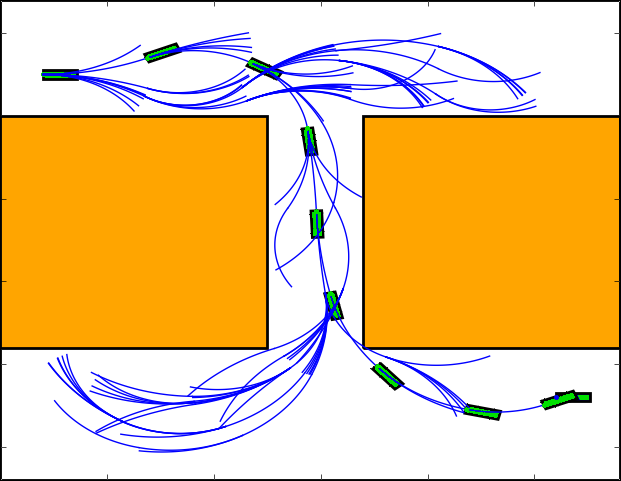
\includegraphics[width=.4\linewidth]{PlannDiffConstr}}
\caption[Comparison between start-to-goal query solutions under geometric and
differential constraints over a 2D workspace.]
{Start-to-goal query solution in a \ac{2D} workspace, where obstacles appear in
orange, free space in white, and the tree of collision-free configurations in
blue. The solution (in green) is calculated by
\protect \subref{fig:PlannGeomConstr_} an \ac{RRT*} under geometric constraints
for a point-like system $\left(\mathcal{C} = \mathbb{R}^{2}\right)$,
and
\protect \subref{fig:PlannDiffConstr} an \ac{RRT} under differential constraints
for a car-like system $\left(\mathcal{C} = \mathbb{R}^2 \times \mathcal{S} \right)$.}
\label{fig:PlannConst}
\end{figure}

There are several successful applications based on this approach. In terrestrial
vehicles, one of the most relevant application was presented by Kuwata \etal
during The DARPA Urban Challenge. They proposed an approach known as
\ac{CL-RRT}, which not only considers the vehicle's motion model, but also
includes the controller's dynamic behavior~\cite{Kuwata2009}. Another
interesting application was done with aerial systems, in which M\"uller \etal
proposed to use an A* for globally finding the collision-free path which, at the
same time, guides an \ac{RRT} expanded under differential constraints.
This latter guarantees finding paths that meet the system's motion
constraints~\cite{Muller2011}.

% ----------------------- subsection  ------------------------
\subsection{Online Path Planning}

As discussed in Chapter~\ref{ch:introduction}, potential and new applications
for \acp{AUV} involve navigating unknown or undiscovered environments that
require endowing the vehicles with the capability of (re)planning online while,
at the same time, they explore the environment. There are different extensions
that can contribute to achieving this requirement, however this section focuses
on two of them. The first is the \textit{anytime} computation, a characteristic
incorporated to different kind of algorithms, including both search-based and
sampling-based methods. The second refers to \textit{lazy collision checking}, a
strategy specifically used with sampling-based methods. These two
characteristics have served as a basis for the proposed approach of this thesis.

% ----------------------- subsubsection  ------------------------
\subsubsection{Anytime Planning Algorithms}

In some situations finding a definite path to solve a start-to-goal query in a
finite and deterministic period of time is not possible. It may occur either
because of the complexity of the task (\ie more computation time is required) or
because vehicles deal with partially known or dynamic environments. In either
case, a common approach is to use an \textit{anytime} algorithm that is capable
of providing the best partial solution when the available time is
over~\cite{Zilberstein1995},\cite{Dean1988}. The most relevant and well-known
planning algorithms have been extended based on this strategy.

Likhachev \etal have studied search-based algorithms, including their extensions
for \textit{anytime} computation. They presented the \ac{ARA*}, a variant that
rapidly calculates a suboptimal path to the goal using a loose bound, which is
later tightened to progressively improve the path~\cite{Likhachev2003}. While
this approach obtains a fast solution, it also permits improving it if
additional time is available. Nonetheless, this approach results useful when
full and accurate information about the environment is available, otherwise it
may require recalculating the whole path if the environment changes. For those
cases, \ie when coping with dynamic environments, it is better to use an
incremental search-based method as \ac{D*}, which allows locally repairing
(replanning) the path when new information of the environment is provided (see
Section~\ref{sec:D-star}). However, in its original version, \ac{D*} lacks the
\textit{anytime} property. In order to improve \ac{D*}'s characteristics,
Likhachev \etal also presented the \ac{AD*}. This is a variant that not only
replans if required, but also improves simultaneously the available solution
path~\cite{Likhachev2005}. A detailed discussion of these \textit{anytime}
search-based algorithms is provided in~\cite{Likhachev2008}.
Some applications for vehicles that not only require online/anytime computation,
but also navigate under motion constraints are also presented
in~\cite{Likhachev2009}.

In the case of sampling-based methods there are also different extensions for
\textit{anytime} computation. Belghith et. al, for example, proposed the
\ac{FADPRM}, which is an approach that combines both: a standard \ac{PRM} for
constructing the roadmap and an \ac{AD*} for finding a solution path. This
latter one extends the original \ac{PRM} by permitting not only \textit{anytime}
calculation, but also a progressive improvement of the resulting path. An
important characteristic of this approach is the possibility to establish zones
with different values of desirability that allow the sampling strategy to be
influenced in order to generate less awkward (inefficient and not smooth)
paths~\cite{Belghith2006}. A similar approach presented by van den Berg
\etal uses \ac{PRM} to represent the static portion of \ac{C-Space} and an
\ac{AD*} to deal with the dynamic elements~\cite{VandenBerg2006}.

On the other hand, and because of its incremental nature, randomized tree-based
methods, such as \ac{RRT}, are more commonly used for applications in partly
known or dynamic environments, where online and \textit{anytime} computation is
required. Ferguson \etal proposed an anytime RRT-based algorithm that calculates
an initial path and its cost using the standard \ac{RRT}, thus ensuring that a
first solution is found in the shortest time possible. Then, a modified \ac{RRT}
iteratively generates a series of new solutions that are guaranteed to have a
lower cost. The algorithm executes until a stop condition is reached, \eg when
the best available solution path needs to be
provided~\cite{Ferguson2006,Ferguson2007}. Other RRT variants as \ac{RRT*} were
also formulated as \textit{anytime} algorithms~\cite{Karaman2011a}.

% Online:
% \cite{Stentz1995}, \cite{Bruce2002}, \cite{Koenig2002}, \cite{Jaillet2004},
% \cite{Maki2009}, \cite{Dolgov2008}, \cite{Kewlani2009}, \cite{Kuwata2009},
% \cite{Likhachev2009}, \cite{Dolgov2010}, \cite{Ardiyanto2011},
% \cite{Muller2011}, \cite{Aoude2013}, \cite{Fulgenzi2009}
% Petti and Fraichard~\cite{Petti2005} presented a tree-based \ac{PMP}, which
% uses limited time slots to obtain updated models of the environment with
% predictions of moving obstacles in order to recalculate the best partial plan.
% First extensions of basic algorithms to support online replanning
% D*~\cite{Stentz1995}, \cite{Koenig2002}, PRM~\cite{Leven2002,Jaillet2004}
% 
% \cite{Likhachev2003}, \cite{Likhachev2005}, \cite{Belghith2006},
% \cite{Karaman2011}, \cite{VandenBerg2006}, \cite{Ferguson2006},
% \cite{Ferguson2007}, \cite{Salzman2013}, \cite{Perez2011},
% \cite{Guibas2009}, \cite{Hornung2013}, \cite{Karaman2010},
% \cite{Likhachev2009}, \cite{Fulgenzi2009}, \cite{Aoude2013},
% \cite{Vannoy2008}, \cite{Karaman2011}, \cite{Jaillet2010},
% \cite{Elbanhawi2014}, \cite{Kurniawati2008}, \cite{Hatton2013}

% ----------------------- subsubsection  ------------------------
\subsubsection{Lazy Collision Checking}
\label{sec:lazy_collision_check}

Even though \ac{PRM} was originally intended for multi-query applications,
Bohlin and Kavraki presented a modified version known as Lazy PRM, which
minimizes the execution time by reducing the quantity of collision checking
callbacks when solving a specific (single) query~\cite{Bohlin2000,Bohlin2001}.
This variant builds a roadmap just as a standard \ac{PRM} does, but it assumes
that all the nodes (configurations) and edges (paths between configurations) are
collision-free, leaving the collision detection to the final stage, \ie when it
must find the shortest path between an initial and a final configuration. If a
collision is found, the associated nodes and edges are discarded (eliminated)
and a new short path is calculated. The authors also suggested an optional
\textit{enhancing roadmap} step when collisions are indeed detected. This
consists in including more samples around the discarded nodes.

This strategy of delaying the collision detection is known as \textit{lazy
collision checking}, and has been used in different applications, especially
those with online computation requirements. Bekris and Kavraki, for instance,
proposed and validated a tree-based planning framework for terrestrial vehicles,
where the states validity is only checked once a path between the start and the
goal configuration has been found~\cite{Bekris2007}. Another example is the one
presented by Vahrenkamp et al., where this strategy was used to speed up the
motions calculation for humanoid robots (with many degrees of freedom, \ie high
dimensional \ac{C-Space})~\cite{Vahrenkamp2007}.

Finally, it is important to note that \textit{lazy collision checking} has
served as a base for one of the extensions proposed and used in this thesis,
which will be explained in detail in Chapter~\ref{ch:plann_online}.

% ----------------------- another section  ------------------------
\section{Path/Motion Planning for AUVs}
\label{sec:StateOfTheArtPlannAUV}

An important aspect to consider when comparing the path/motion planning
approaches for \acp{AUV} is their application. Based on this, the different
contributions can be classified into two main categories. The first group
gathers those applications that require \acf{CPP} techniques, which are commonly
applied to guide \acp{AUV} over survey tasks. The most common examples within
this group include coverage missions used for creating in detail bathymetric
maps of the seabed~\cite{Fang2010, Galceran2012, Galceran2013b, Galceran2013d},
detecting potential targets (such as underwater mines~\cite{Stack2003,
Williams2010}) and inspecting artificial structures (such as in-water ship
hulls~\cite{Englot2010, Hover2012, Hollinger2013, Englot2013}), as well as
natural marine formations~\cite{Galceran2014,Galceran2014b}.

A common characteristic in all these approaches is that the planner is provided
with preliminary information of the target area or structure (see
Fig.~\ref{fig:CPP-App}). This may include its location and shape. Based on this,
the \ac{CPP} algorithm defines a survey path that, in some cases, is reshaped or
refined online according to the data obtained during the mission execution. This
characteristic implies that most of the computation is done offline, \ie before
conducting the mission. Most recent work presented by Vidal \etal proposes a
novel approach to conduct inspection tasks without preliminary information of
the target. Results are, however, still limited to \ac{2D} motions (at a
constant depth)~\cite{Vidal2017}.

\begin{figure}[htbp]
    \myfloatalign
    \subfloat[Coverage path over of a natural formation. Image credit: Galceran
    \etal\cite{Galceran2013b}]
    {\label{fig:CPP-NaturalFormation}
    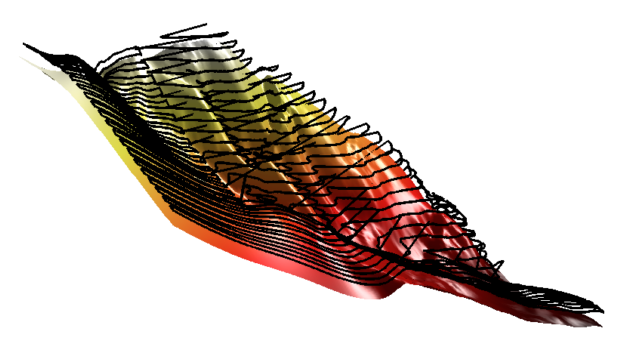
\includegraphics[width=.5\linewidth]{CPP-NaturalFormation}} \\
    \subfloat[Coverage path of a ship hull. Image credit: Hover
    \etal\cite{Hover2012,Englot2013}] 
    {\label{fig:CPP-ShipHull}%
     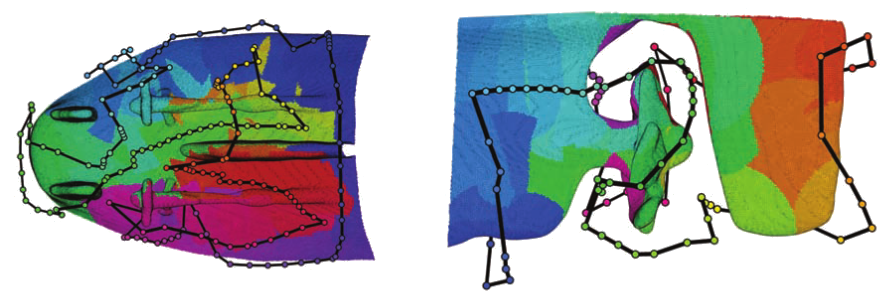
\includegraphics[width=.90\linewidth]{CPP-ShipHull}}
\caption[Coverage path planning (CPP) applications.]
{Coverage path planning (CPP) algorithms are normally used to plan routes to
inspect different kind of structures. In most of these applications the planner
has preliminary information. This may include a 2D/3D map of the area or
structure to be inspected.}
\label{fig:CPP-App}
\end{figure}

The second group of \ac{AUV} applications, on the other hand, gathers those that
are focused on safely and efficiently guiding the vehicle from one initial
position to a specified goal. For doing so, different strategies, such as those
explained throughout previous sections, have been applied to underwater
vehicles. In fact, these start-to-goal methods are commonly used as low-level
motion planners required for the aforementioned coverage applications. The work
presented throughout this thesis seeks to make contributions to this group of
start-to-goal applications, therefore it is important to identify the main
characteristics between the different approaches used.

\subsection{2D and 3D Planning for Propeller-driven Vehicles}

A first characteristic, and one that is not obvious immediately is the
capability of conducting \ac{2D} and \ac{3D} motions. Although \acp{AUV}
operate in \ac{3D} workspaces, in a significant number of applications the
vehicles navigate either at a constant altitude or at a constant
depth~\cite{Carroll1992,Sequeira1994,Vasudevan1994,Arinaga1996,Petillot2001,Kawano2002,Alvarez2004,Hong-jian2004,Tan2004,Garau2005,Kruger2007,Petres2007,Yilmaz2008,Soulignac2009,Caldwell2010,Cheng2010,Poppinga2011,Soulignac2011,Kim2012a,McMahon2016},
thus considerably simplifying the motion planning problem. There are, however,
some contributions that have presented alternatives in modelling and planning
\ac{3D} (and therefore \ac{2D}) \ac{AUV} motions. Considering these latter ones,
it is still necessary to make a distinction between those approaches used for
underwater gliders~\cite{Smith2010,Thompson2010,Wehbe2014,Cao2016}, and those
used for propeller-driven \acp{AUV} (as the ones in this
work)~\cite{Warren1990,Sugihara1997,Qu2009,Murthy2010,Yan2012,Heo2013,Taleshian2015,Ni2016}.

In both cases, \ie \ac{2D} and \ac{3D} motions, path/motion planning
alternatives for propeller-driven \acp{AUV} make use of different approaches
such as potential fields~\cite{Warren1990,Sequeira1994}, genetic
algorithms~\cite{Sugihara1997,Alvarez2004,Hong-jian2004}, as well as
sensor-based~\cite{Ying2000,Houts2012},
grid-based~\cite{Sequeira1994,Arinaga1996,Carroll1992,Garau2005,Rao2009,Yan2012,Kim2012a},
and sampling-based
methods~\cite{Tan2004,Rao2009,Caldwell2010,Poppinga2011,Heo2013,McMahon2016}.
However, in some of these situations, the vehicle operates in open sea areas
(see Fig.~\ref{fig:GlidersMissions}), where they do not usually have to deal
with obstacles, narrow passages, or high-relief environments. This is the case
for the new potential applications presented in Chapter~\ref{ch:introduction}.
In such situations, the planner must at least consider the vehicle's motion
capabilities.

\begin{figure}[htbp]
    \myfloatalign
    \subfloat[Glider sinusoidal-like vertical motion. Image credit: Thompson
    \etal\cite{Thompson2010}]
    {\label{fig:GlidersMissions3D}
    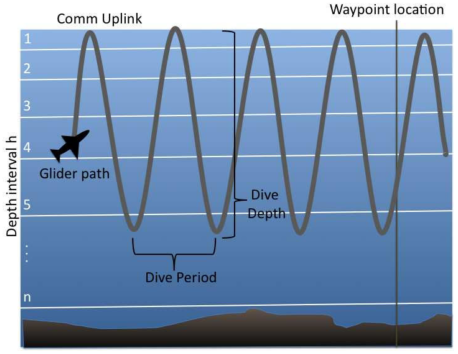
\includegraphics[width=.48\linewidth]{GlidersMissions3D}} \quad
    \subfloat[Glider one-month-long mission. Image credit: Smith
    \etal\cite{Smith2010}] 
    {\label{fig:GlidersMissionsTop}%
     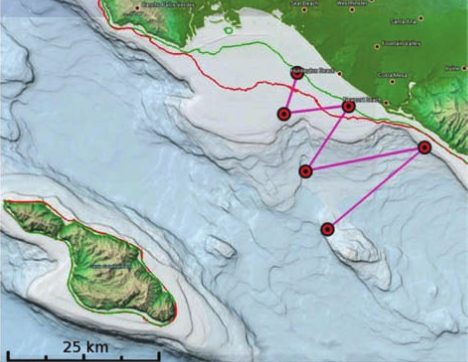
\includegraphics[width=.48\linewidth]{GlidersMissionsTop}}
\caption[Examples of underwater gliders missions.]
{\protect \subref{fig:GlidersMissions3D} Due to their propulsion mechanisms,
underwater gliders normally follow sinusoidal-like trajectories.
\protect \subref{fig:GlidersMissionsTop} They conduct long-term missions
and operate in open sea and obstacle-free areas.}
\label{fig:GlidersMissions}
\end{figure}

\subsection{Path Planning for Motion-constrained Vehicles}

A second characteristic required in analyzing and comparing different planning
approaches for the intended applications mentioned in
Chapter~\ref{ch:introduction}, is the capability of generating feasible paths,
\ie paths that meet the vehicles' motion constraints (see
Section~\ref{sec:motion_constraints_review}). A first group includes those
approaches that use sensor-based methods either to navigate through unknown
underwater environments~\cite{Ying2000}, or to follow the terrain shape of a
given bathymetric map~\cite{Houts2012} (see
Fig.~\ref{fig:SensorBasedConstrainedAUV}). In both cases, the vehicle is assumed
to be equipped with a forward-looking sonar to reactively avoid collisions. Such
maneuvers are calculated by a local planner that meets the \ac{AUV} kinematics
or dynamics. An important characteristic of this kind of approach is the lack of
global knowledge of the environment (\ie a map is not incrementally built),
which can cause the vehicle to get trapped in complex scenarios.

\begin{figure}[htbp]
    \myfloatalign
    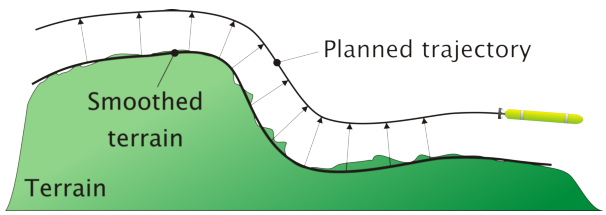
\includegraphics[width=.85\linewidth]{SensorBasedConstrainedAUV}
\caption[Sensor-based planning for AUVs under motion constraints.]
{Sensor-based planning for AUVs under motion constraints. The vehicle trajectory
can be either preplanned or incrementally calculated to maintain a desired
distance from the terrain. The resulting trajectory is fit to satisfy
curvature constraints that approximate the AUV motion constraints. Image credit:
Houts \etal\cite{Houts2012,Houts2014}.}
\label{fig:SensorBasedConstrainedAUV}
\end{figure}

A similar reactive approach establishes a set of inequality constraints that
describe the obstacles as convex regions contained in the \ac{C-Space}.
Moreover, the initial configuration is treated as the starting point of a
nonlinear search, where the goal configuration is assumed to be a unique global
minimum of the objective function. The start-to-goal query is then solved as an
optimization problem, in which a local planner takes into account the vehicles'
constraints. This strategy was one of the first online obstacle avoidance
approaches for underwater vehicles; it used a real-world dataset of acoustic
images obtained by a \ac{ROV} equipped with a multibeam forward-looking sonar.
Its validity was demonstrated by guiding a simulated \ac{ROV}. However, the
capability of simultaneous mapping (detection) and planning online was not
proven~\cite{Petillot2001}.

The formulation that represents obstacles as convex regions has likewise been
used either to represent obstacles detected online, which trigger collision
avoidance maneuvers~\cite{Qu2009}, or to approximate the terrain shape that must
be followed by the vehicle~\cite{Murthy2010}. In both cases, the low-level
controller attempts to generate feasible (doable) trajectories by using the
\ac{AUV} kinematic equations and spline-based interpolation techniques,
respectively. However, the main drawback of these approaches is the difficulty
in creating a convex representation of complex obstacles.

Another common strategy used in some of the aforementioned methods, is
mathematically making the solution paths more suitable for a motion-constrained
\ac{AUV}. Pêtrès et al., for instance, proposed a \ac{FM}-based approach to find
collision-free paths, which are smoothed by a cost function that contains
kinematic and curvature constraints~\cite{Petres2007} (see
Fig.~\ref{fig:CostFunctionConstrainedAUV}). Likewise, another example based on
\acp{GA} finds a valid route to the goal by using \ac{B-spline} curves, thus
seeking to generate more feasible trajectories for \acp{AUV}~\cite{Cheng2010}.


\begin{figure}[htbp]
    \myfloatalign
    \subfloat[]
    {\label{fig:CostFunctionConstrainedAUV-a}
    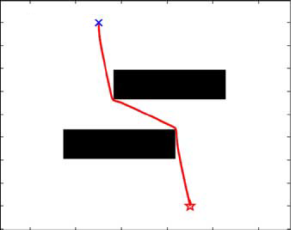
\includegraphics[width=.3\linewidth]{CostFunctionConstrainedAUV-a}} \quad
    \subfloat[] 
    {\label{fig:CostFunctionConstrainedAUV-b}%
     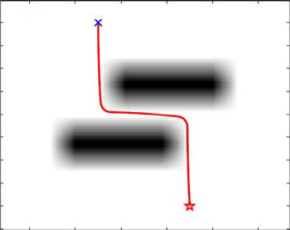
\includegraphics[width=.3\linewidth]{CostFunctionConstrainedAUV-b}} \quad
     \subfloat[] 
    {\label{fig:CostFunctionConstrainedAUV-c}%
     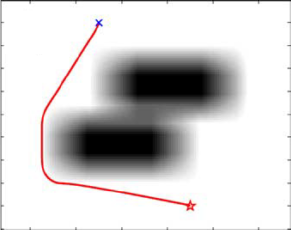
\includegraphics[width=.3\linewidth]{CostFunctionConstrainedAUV-c}}
\caption[FM-based planning for AUVs under motion constraints.]
{Start-to-goal query that is solved by a FM-based method. The solution path is
smoothed by a cost function to approximate the AUV motion constraints.
\protect \subref{fig:CostFunctionConstrainedAUV-a} The initial optimal path.
\protect \subref{fig:CostFunctionConstrainedAUV-b} The effect after smoothing the
path.
\protect \subref{fig:CostFunctionConstrainedAUV-c} The use of the cost function
can merge the obstacles, thus discarding possible solutions. Image credit:
Pêtrès \etal\cite{Petres2007}.}
\label{fig:CostFunctionConstrainedAUV}
\end{figure}

There is another group that gathers different grid-based approaches. Sequeira
and Ribeiro, for example, presented a two-layer framework that is composed of a
\ac{HLP} and a \ac{LLP}. The \ac{HLP} creates a visibility graph using the
information of the known obstacles, sea currents, and specified waypoints of the
mission. Furthermore, the energy required to move between the graph nodes
corresponds to the edge weights. The global and optimal geometric route to the
goal is then found by Dijkstra's algorithm. Finally, in order to calculate the
vehicle's maneuvers between the different solution segments, the \ac{LLP} uses
an \ac{AFP}. This way the total artificial force includes a \ac{3D} double
integrator that takes into account the \ac{AUV} motion
constraints~\cite{Sequeira1994}. There are other similar two-layer approaches,
where the global path planning problem is tackled with a grid-based method, and
the local motion planning deals with the \ac{AUV}
constraints~\cite{Arinaga1996} (see Fig.~\ref{fig:GridBasedLocalConstrAUV}). The
main disadvantage of this approach is that the grid-based layer generally
requires \textit{a priori} information of the environment, \eg a navigation map.

\begin{figure}[htbp]
    \myfloatalign
    \subfloat[]
    {\label{fig:GridBasedLocalConstrAUV-a}
    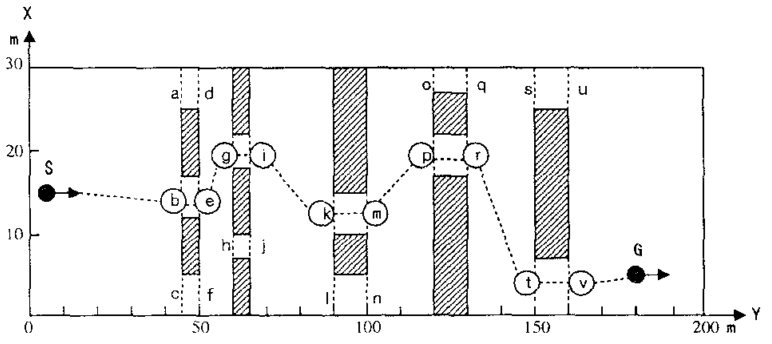
\includegraphics[width=.55\linewidth]{GridBasedLocalConstrAUV-a}} \quad
    \subfloat[] 
    {\label{fig:GridBasedLocalConstrAUV-b}
     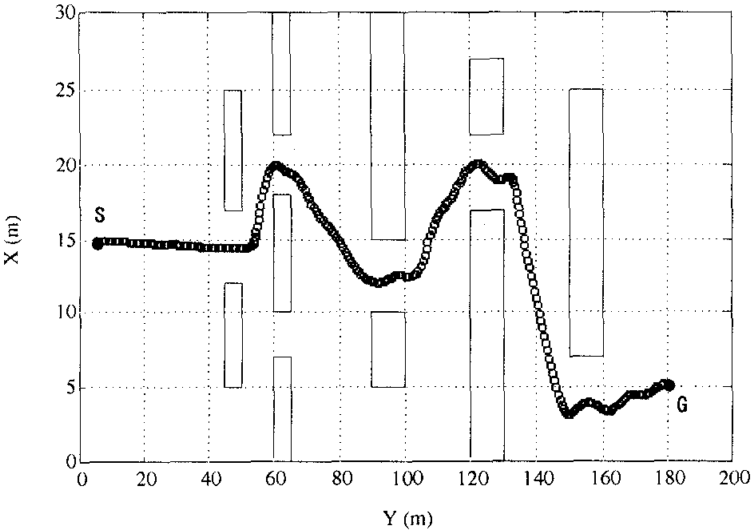
\includegraphics[width=.4\linewidth]{GridBasedLocalConstrAUV-b}}
\caption[Combination of a grid-based planning method and a local planner
to include the AUV motion constraints.]
{\protect \subref{fig:GridBasedLocalConstrAUV-a} Global path planning solved by
a grid-based method, \protect \subref{fig:GridBasedLocalConstrAUV-b} which is
adjusted by a local planner that takes into consideration the AUV motion
constraints. Image credit: Arinaga \etal\cite{Arinaga1996}.}
\label{fig:GridBasedLocalConstrAUV}
\end{figure}

A group of recent contributions includes those that use sampling-based planning
algorithms. The most common approach builds a tree of collision-free
configurations, which are obtained by integrating the differential equation that
describes the \ac{AUV} dynamic behavior~\cite{Tan2004,Caldwell2010,Heo2013}.
This strategy was briefly introduced in
Section~\ref{sec:motion_constraints_review}, but its use with a torpedo-shaped
\ac{AUV} will be explained in more detail in
Chapter~\ref{ch:motion_constratins}.

Finally, there is a geometric alternative to generate feasible paths for
motion-constrained \acp{AUV}. It consists in utilizing the Dubins
paths~\cite{Dubins1957}, which establishes a set of six maneuvers (RSR, RSL,
LSR, LSL, RLR, LRL, where R states for Right, L for Left, and S for straight) to
connect two configurations $q_i,q_j \in \mathcal{C} = SE(2)$. It has been
typically used with car-like systems, and more recently with some underwater
vehicles~\cite{Wehbe2014,Cao2016} (see Fig.~\ref{fig:Dubins3DGlidersConstrAUV}).
However, in this latter case, the Dubins paths have worked more as a trajectory
planner, rather than a path planner with online obstacle avoidance capabilities.
Further discussion of Dubins maneuvers and their use with \acp{AUV} will be
presented throughout
Chapters~\ref{ch:motion_constratins}~and~\ref{ch:planning_3D}.

\begin{figure}[htbp]
    \myfloatalign
    \subfloat[]
    {\label{fig:Dubins3DGlidersConstrAUV-a}
    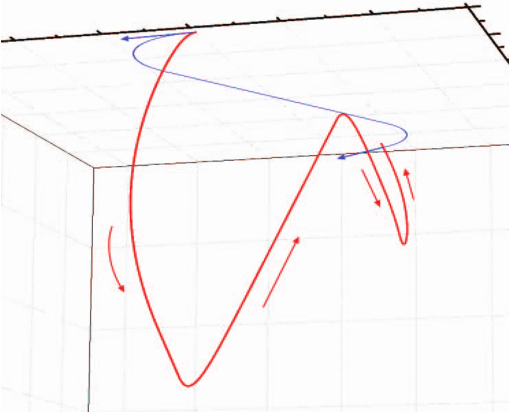
\includegraphics[width=.45\linewidth]{Dubins3DGlidersConstrAUV-a}} \quad
    \subfloat[] 
    {\label{fig:Dubins3DGlidersConstrAUV-b}
     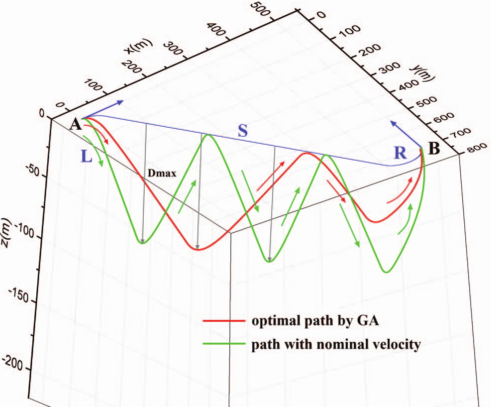
\includegraphics[width=.45\linewidth]{Dubins3DGlidersConstrAUV-b}}
\caption[Glider trajectory planner combining the Dubins curves and
sinusoidal-like vertical motion.]
{\protect \subref{fig:Dubins3DGlidersConstrAUV-a} Glider trajectory planner that
combines the Dubins curves and the sinusoidal-like vertical motion.
\protect \subref{fig:Dubins3DGlidersConstrAUV-b} A genetic algorithm calculates
the optimal trajectory for a glider that moves in obstacle-free environment.
Image credit: Cao \etal\cite{Cao2016}.}
\label{fig:Dubins3DGlidersConstrAUV}
\end{figure}

\subsection{Online Mapping and Path/Motion Planning}

As mentioned in the introduction of this manuscript, one alternative in coping
with the restrictions imposed by the new and potential applications for
\acp{AUV} is to endow the vehicles with the capability of navigating through
unknown or unexplored environments. For doing so, it is necessary that the
vehicle can (re)plan its own motions while exploring the surroundings. However,
little research has addressed this problem of mapping and planning safe routes
simultaneously and online for \acp{AUV}. Apart from the already explained work by
Petillot et al., which in fact does not prove online mapping and planning
capacity~\cite{Petillot2001}, Maki \etal~proposed an online path planning method
that uses landmarks to guide an \ac{AUV}. Nonetheless, their approach does not
permit replanning and, furthermore, results were obtained in a controlled
environment (\ie in a water tank)~\cite{Maki2007}.

This chapter has presented an extensive review of the most common path/motion
planning approaches, and those that have been used with underwater vehicles. The
following chapters will present the extension of some of these approaches, and
their successful use in some of the intended applications introduced in
Chapter~\ref{ch:introduction}.

% ---------------------------------------------------------------------------
% ----------------------- end of thesis sub-document ------------------------
% ---------------------------------------------------------------------------